
\section{Sampling} \label{sec:sampling}
\subsection{Geometry}
Shown in Figure \ref{fig:conops}, 
% the origin of the body frame is with the coordinate system defined by triad vectors $\hat{\mathbf{y}}_b$, $\hat{\mathbf{x}}_b$, and $\hat{\mathbf{z}}_b$ that in respective order point along the largest to the smallest principal inertia axes. 
the triad axes $\hat{\mathbf{x}}_b$, $\hat{\mathbf{y}}_b$ and $\hat{\mathbf{z}}_b$ represent the body frame that rotates in orbit. The refraction axis of the hyperspectral imager  is mounted along the $\hat{\mathbf{z}}_b$ axis, the slit height $h_\text{slit}$ is mounted along the $\hat{\mathbf{y}}_b$ axis and the slit width $w_\text{slit}$ is mounted along the $\hat{\mathbf{x}}_b$ axis. The satellite's orbit frame where $\hat{\mathbf{x}}_o$ points along the velocity vector (along-track), $\hat{\mathbf{y}}_o$ points towards the negative orbit normal vector (cross-track), $\hat{\mathbf{z}}_o$ represents the nadir vector which is aligned with the position vector defined in the Earth-Centered-Inertial (ECI) frame. 
% The 2-D reference frame of a pixel on ground is represented with $\Delta x$ and $\Delta y$, being in-track and cross-track resolution respectively.
The rotation of the satellite body relative to the orbit may be represented by the Euler angles $\phi$, $\theta$ and $\psi$ which are the roll, pitch and yaw angles. In addition, the absolute angle between the Line-of-Sight (LOS) vector $\boldsymbol{\rho}$ and $\hat{\mathbf{z}}_o$, is defined as the viewing angle $\gamma$.
% \begin{align}
% \gamma &=\cos^{-1}\left(\frac{1}{\sqrt{\sec^2(\theta)+\tan^2(\phi)}}\right)
% \end{align}
% 
The angular velocities about the satellite body frame, as measured by on-board gyroscope sensors, are represented by $\omega_x$, $\omega_y$, and $\omega_z$. 

% The transformation is undefined for $\theta = \pm \frac{\pi}{2} \pm q \pi$ where $q$ is an integer.\footnote{In practice, it is assumed that the singularity is avoided by imposing $\vert\theta\vert<\frac{\pi}{2}$ during a slew maneuver about the $\hat{\mathbf{y}}_b$ axis as the concerned remote sensing targets are beneath the orbit track and not at or beyond the Earth's horizon.}
The hyperspectral imager's instantaneous footprint, expressed in horizontal and vertical components, are
% \begin{subequations}
% \begin{align}
% P_{w} &= H\sin\Big(\frac{\epsilon_{w}}{2}\Big)\sec\phi\sec\theta \Bigg(\sec\Big(\theta+\frac{\epsilon_w}{2}\Big)\notag\\&+\sec\Big(\theta-\frac{\epsilon_w}{2}\Big)\Bigg), \\
% P_{h} &= H\sin\Big(\frac{\epsilon_{h}}{2}\Big)\sec\theta\sec\phi\Bigg(\sec\Big(\phi+\frac{\epsilon_h}{2}\Big)\notag\\&+\sec\Big(\phi-\frac{\epsilon_h}{2}\Big)\Bigg),
% \end{align}
% \end{subequations}
\begin{subequations}
\begin{align}
P_{w} &= H\sec\phi\bigg(\tan\Big(\theta+\frac{\epsilon_w}{2}\Big)-\tan\Big(\theta-\frac{\epsilon_w}{2}\Big)\bigg), \\
P_{h} &= H\sec\theta\bigg(\tan\Big(\phi+\frac{\epsilon_h}{2}\Big)-\tan\Big(\phi-\frac{\epsilon_h}{2}\Big)\bigg),
\end{align}
\end{subequations}
\noindent which are transformed to the along-track and cross-track components of a central pixel as
\begin{subequations}
\begin{align}
\delta x &\triangleq \cos(\psi)P_{w}+\sin(\psi)\frac{P_{h}}{N_{y}}, \label{eq:footprint_x}\\
\delta y &\triangleq \cos(\psi)\frac{P_{h}}{N_{y}}-\sin(\psi)P_w. \label{eq:footprint_y}
\end{align}
\end{subequations}
Ground-projected pixels near the edge of the swath are elongated compared to the central pixel. Along with effects from Earth curvature, this distortion is known as the "bowtie effect" which may be corrected in image processing \cite{Richards1999, Sayer2015}. We note that the ground pixel size is relatively small (i.e. on a meter-scale) and the combination of high frame rate and narrow FoV renders the pixel elongation and the Earth curvature as seen per pixel to be practically negligible.
\subsection{Spatial Resolution}
Using Eqs. (\ref{eq:footprint_x}) and (\ref{eq:footprint_y}), then the spatial resolution in a pixel acquired during exposure time $\tau$, as shown conceptually in Figure \ref{fig:push_scan}, are expressed in along-track and cross-track components as
\begin{subequations}
\begin{align}
    \Delta x=\delta x+v_{p,x}\tau, \label{eq:spatial1_x} \\
    \Delta y=\delta y +v_{p,y}\tau, \label{eq:spatial1_y}
\end{align}
\end{subequations}
\noindent where $v_{p,x}$ and $v_{p,y}$ are the along-track and cross-track pixel speed as measured on ground
\begin{subequations}
\begin{align}
    v_{p,x} & \triangleq v_{o}
+\dot{\theta}H-\dot{\psi}H\tan(\phi), \label{eq:rotational_vel1} \\
    v_{p,y} & \triangleq -\dot{\phi}H+\dot{\psi}H\tan(\theta), \label{eq:rotational_vel2}
\end{align}
\end{subequations}
\noindent with $v_o$ being the speed of the satellite as measured on ground. 
% The Earth ground speed $v_g$ results in moving features in an image pixel due to the Earth's rotational rate and decreases with higher geodetic latitude of the target area. The Relative Ground Shift (RGS) during a camera exposure time takes into account the relative motion between moving footprint and ground and may be determined by adding the Earth surface speed in the along-track and cross-track distances covered such that $(v_{p,x}-v_{g,x})\tau $ and $(v_{p,y}-v_{g,y})\tau $, respectively. RGS is indicative of motion blur and determines how much a pixel and a surface feature has shifted on ground during an exposure.
\begin{figure}[htbp]
  \begin{center}
    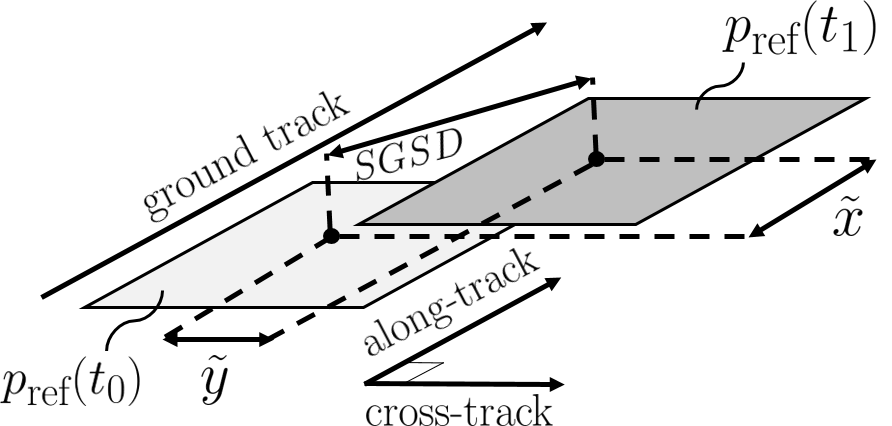
\includegraphics[width=70mm,angle=0]{figs/SGSD.png}
    \caption{Illustration of how SGSD is defined. $p_{\text{ref}}(t_1)$ and $p_{\text{ref}}(t_0)$ denote the reference pixel at time $t_1$ and $t_0$, respectively.} 
    \label{fig:SGSD}
\end{center}
\end{figure}
% The read-out distance, i.e. the distance covered between closing camera shutter and opening it again to capture the next frame, are defined in along-track and cross-track components as $v_{p,x}\delta t$ and $v_{p,y}\delta t$, respectively. In an ideal scenario for a pushbroom imager scanning uniformly in the along-track direction, the cross-track SGSD is zero, i.e. $\tilde{y}=0 \hspace{3pt} \rm{m}$ during $\Delta t = t_1-t_0$. 
Shown in Figure \ref{fig:SGSD}, the SGSD may therefore be defined as the distance between two sequential reference pixels during a camera integration time $\Delta t$, expressed by  along-track and cross-track components, as
\begin{subequations}
\begin{align}
    \tilde{x} & \triangleq v_{p,x}\Delta t, \label{eq:SGSD1} \\
    \tilde{y} & \triangleq v_{p,y}\Delta t. \label{eq:SGSD2}
\end{align}
\end{subequations}
The SGSD also determines the amount of overlap in the set of frames. If the scan direction is aligned with the velocity vector, and since the satellite has high speed as well as $\delta x$ being significantly larger than $\delta y$, it is preferred to slew about the $\hat{\mathbf{y}}_b$ axis to enable better along-track spatial resolution. From Eqs. (\ref{eq:rotational_vel1}) and (\ref{eq:rotational_vel2}) the required angular velocity of the satellite $\omega_{y}$ may be obtained from setting the desired SGSD and vice versa. Alternatively, $\omega_{y}$ and SGSD can be set if a a fixed target length shall be uniformly scanned. 
% if pitch angles at the start and at the end of image acquisition are equal in magnitude but of oppsite sign.
% The required angular velocities for selected integration times are shown in Figure \ref{fig:gsd_desired}.
% \begin{figure}[htbp]
%   \centering
%       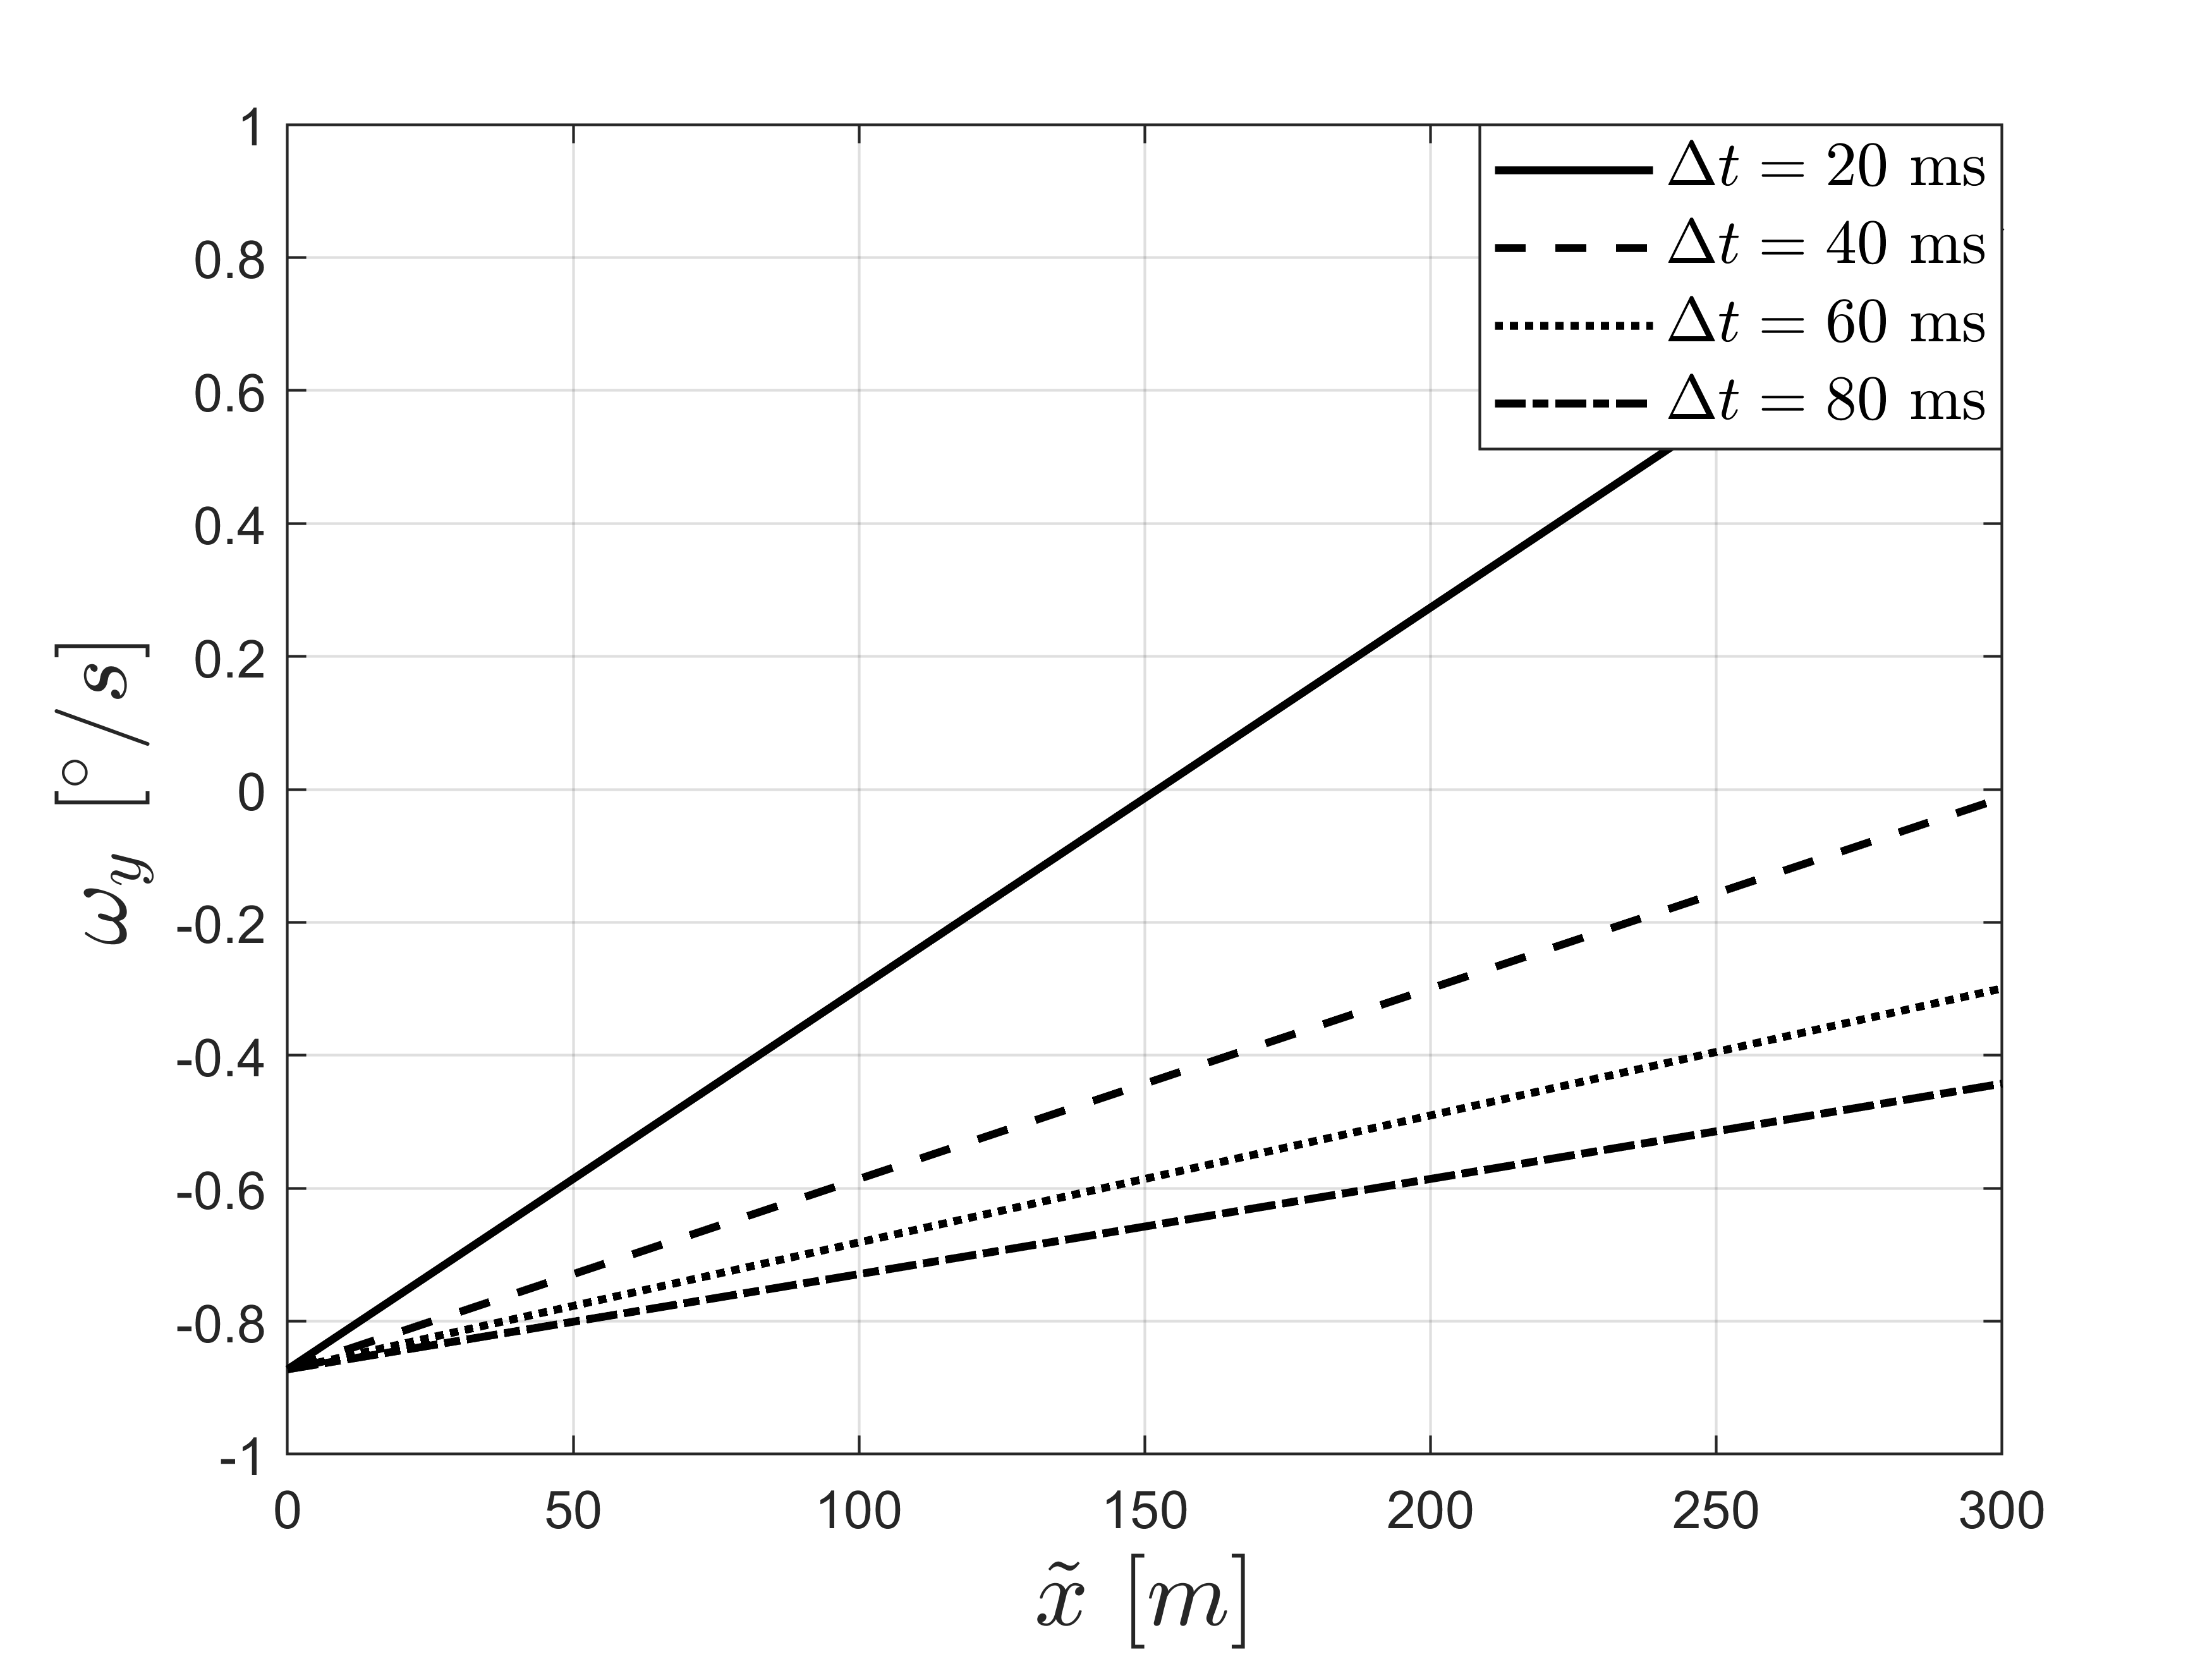
\includegraphics[width=0.48\textwidth]{figs/ang_vel_ref.png}
%   \caption{Reference angular rate $\dot{\theta}=\omega_{y}$ vs. desired along-track SGSD assuming $\omega_x=\omega_z=0$, for different integration times $\Delta t$. Altitude is $H=500 \hspace{3pt} \rm{km}$.}
% 	\label{fig:gsd_desired}
% \end{figure}
% \subsection{Slew Maneuver Strategies}
% \subsubsection{GSD-Driven Slew Maneuver}
% Suppose constant and small $\Delta t>0$, $\omega_{x}=\omega_{z}=0$, and $\psi=0$. Re-arranging Eqs. (\ref{eq:rotational_vel1}), the angular velocity of the satellite may be chosen from desired instantaneous in-track GSD $\tilde{x}_{\text{ref}}$ as
% \begin{align}
% \dot{\theta}_{\text{ref}} &= \frac{1}{H}\Big(v_{s}-v_{g,x}+\frac{\tilde{x}_{\text{ref}}}{\Delta t}\Big). \label{eq:desired_inst_gsd_x}
% \end{align}
\subsection{Imaging Strategy} 
Consider the length $s_{g}$ that shall be observed during the time $\Delta T=t_f-t_0$ and the satellite rotating from start to end pitch angles $\theta(t_0)=\theta_0$ and $\theta(t_f)=\theta_f$. Assuming constant altitude, to uniformly scan the target the final pitch angle may be set to $\theta_f=-\theta_0$ such that $\delta x(t_0)=\delta x (t_f)$. The geometry is shown in Figure \ref{fig:orbit-track}. Furthermore, it is assumed that $\omega_{z} = \omega_{x} = 0$, $\phi=\psi=0$ such that $\omega_y=\dot{\theta}$. 
\begin{figure}[htbp]
  \centering
      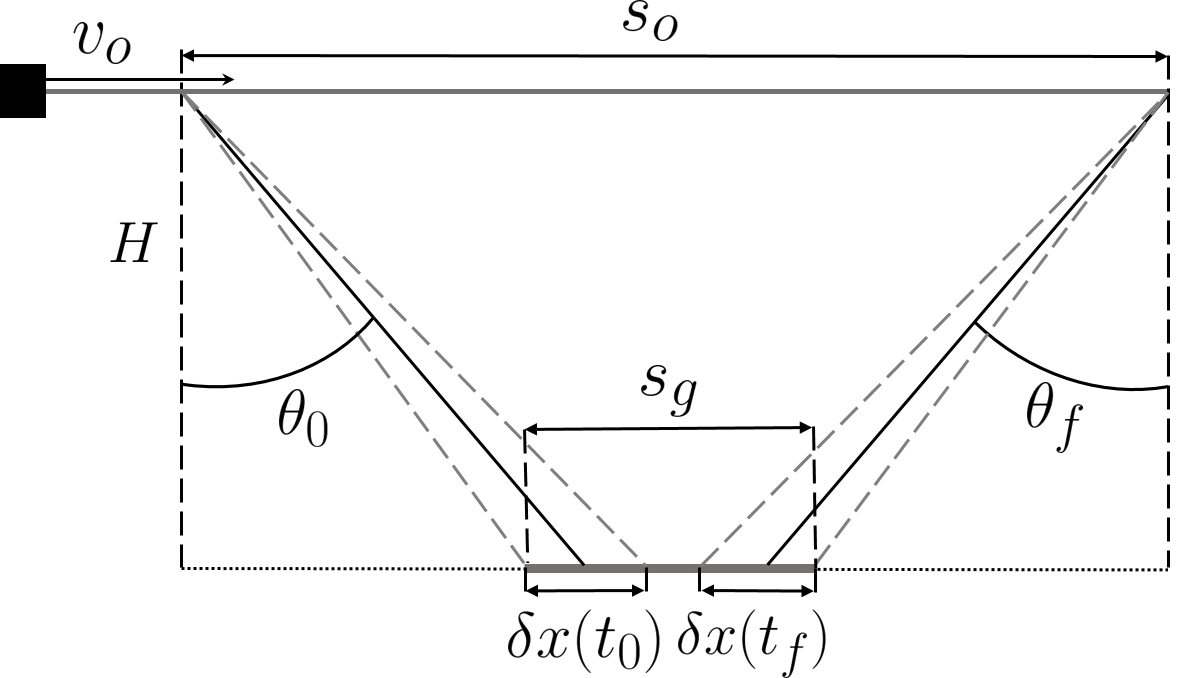
\includegraphics[width=0.45\textwidth]{figs/orbit_track.png}
  \caption{Geometry of a satellite slewing across a ground target with objective to acquire images along the distance $s_g$. Altitude is $H=500 \hspace{3pt} \rm{km}$.}
	\label{fig:orbit-track}
\end{figure}
The orbit track can be calculated as
\begin{align}
s_{o}&=s_{g}+H\Bigg(\tan\bigg(\theta_0-\frac{\epsilon_{w}}{2}\bigg)-\tan\bigg(\theta_f-\frac{\epsilon_{w}}{2}\bigg)\Bigg).
\end{align}
The time $\Delta T$ required to perform the slew maneuver, can be calculated as
\begin{align}
\Delta T & = \frac{s_{o}}{v_{o}},
\end{align}
and the angular velocity of the spacecraft may found from
\begin{equation}
\omega_{y}=\dot{\theta} = \frac{\Delta \theta}{\Delta T}.
\end{equation}
Figure \ref{fig:slew_angle} shows required angular velocity $\omega_y$ as a function of $\theta_0=-\theta_f$ for varying length $s_g$ to be observed.
\begin{figure}[htbp]
  \centering
      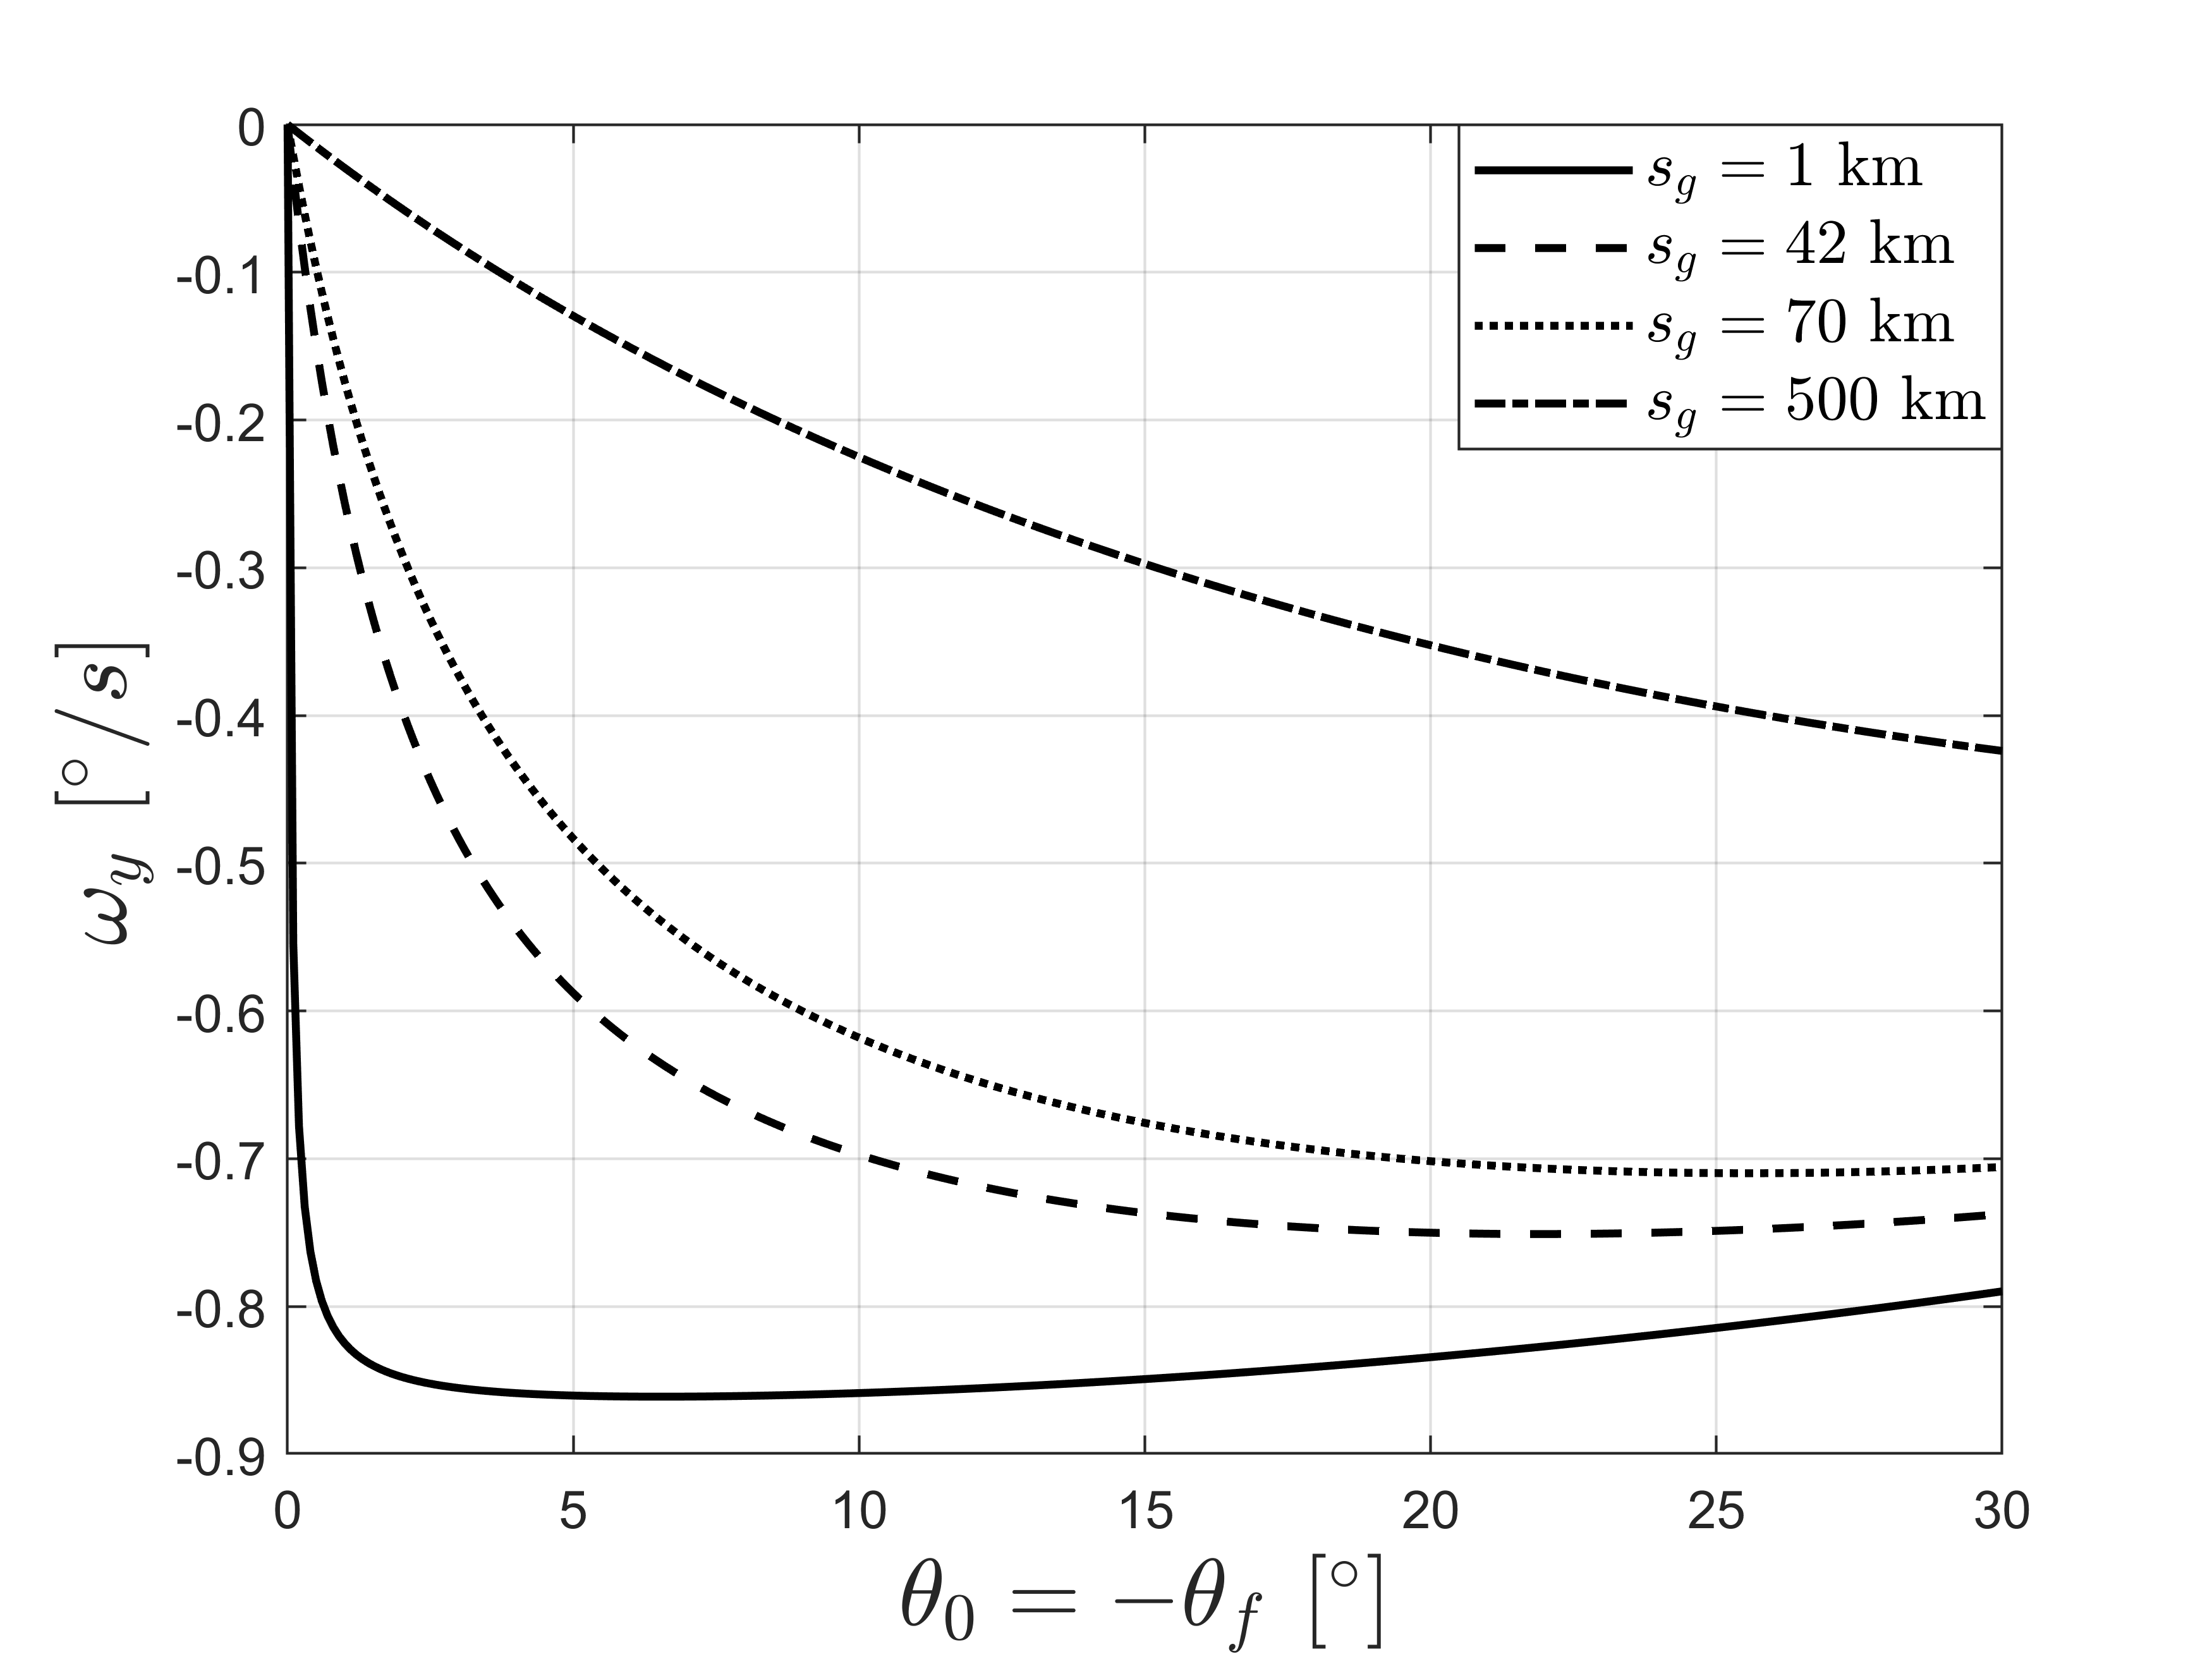
\includegraphics[width=0.48\textwidth]{figs/ang_vel_track.png}
  \caption{Angular velocity $\omega_{y}$ vs. pitch angles $\theta_0=-\theta_f$ for different $s_g$. Altitude is $H=500 \hspace{3pt} \rm{km}$.}
	\label{fig:slew_angle}
\end{figure}
\subsection{Expected Performance}
\subsubsection{Resolution for Nadir-pointing} \label{sec:spacecraft_nadir} 
\begin{table}[htbp]
	\caption{Simulation parameters}
	\label{tab:camera_params}
	\centering
			\begin{tabular}{l r}
				\hline
                Parameter & Value \\
                \hline
                FPS & 22 \\ 
                Camera Integration time $\Delta t$ & $45.4 \hspace{3pt} \rm{ms}$ \\
                Camera Exposure time $\tau$ & $41.4 \hspace{3pt} \rm{ms}$ \\
                Camera Read-out time $\delta t$ & $4 \hspace{3pt} \rm{ms}$ \\
                Target length $s_g$ & $40.08 \hspace{3pt} \rm{km}$ \\
                Altitude $H$ & $500 \hspace{3pt} \rm{km}$ \\
                Satellite speed $v_o$ & $7.61 \hspace{3pt} \rm{km/s}$ \\
                Roll angle $\phi$ & $0^{\circ}$ \\
                Yaw angle $\psi$ & $0^{\circ}$ \\
				\hline
				\end{tabular}
\end{table}
With hyperspectral imager's scan direction being aligned with the along-track direction while pointing at nadir, i.e. $\theta=0^{\circ}$, its instantaneous pixel resolution is $\delta x =500 \hspace{3pt} \rm{m}$. Using the specifications in Table \ref{tab:optics} and camera settings in Table \ref{tab:camera_params}, the obtained spatial resolution is $\Delta x = 815.6 \hspace{3pt} \rm{m}$, $\Delta y =58.6 \hspace{3pt} \rm{m}$ and a swath width of $P_{h}=40.08 \hspace{3pt} \rm{km}$. The along-track SGSD becomes $\tilde{x} =346 \hspace{3pt} \rm{m}$, meaning that $3$ frames partially overlap. It takes $\Delta T = 5.23 \hspace{3pt} \rm{s}$ to scan a target length of $s_g=s_o=40.08 \hspace{3pt} \rm{km}$.
\subsubsection{Resolution for Slew Maneuver} \label{sec:spacecraft_slew}
Using the same parameters in Tables \ref{tab:optics} and \ref{tab:camera_params} are used for imaging during a slew maneuver, Figures \ref{fig:spatial_time} and \ref{fig:cross_spatial_time} show how spatial resolution varies with different pitch rates in ideal settings where no attitude errors are present. Table \ref{tab:SGSD} shows the corresponding SGSD, reference angular velocity and duration for each starting pitch angle $\theta_0$. For example with $\theta_0=20^{\circ}$ as starting pitch angle, the satellite would have to slew at a reference angular velocity of $\omega_{y}= -0.754^{\circ}/\rm{s}$ for $\Delta T = 53.05 \hspace{3pt} \rm{s}$ to cover the target length $s_g=40.08 \hspace{3pt} \rm{km}$ uniformly. The spatial resolution varies between $\Delta x=609.2 \hspace{3pt} \rm{m}$ at $\theta=20^{\circ}$ to $\Delta x= 542.9 \hspace{3pt} \rm{m}$ at $\theta=0^{\circ}$. Additionally, a SGSD of $\tilde{x} = 47.09 \hspace{3pt} \rm{m}$ is achieved instead of $\tilde{x} = 346 \hspace{3pt} \rm{m}$ for the nadir-pointing case. This means there will be at least $12$ frames that partially overlap in the along-track direction, instead of $3$ for nadir-pointing. 

In reality, due to attitude stabilization inaccuracies and system noise, the spatial resolution and SGSD will vary significantly throughout the image acquisition. With reference to the image resolution requirement discussed in Section \ref{sec:mission-design}, in order to have a sequential pixel-to-pixel distance to be less than $100 \hspace{3pt} \rm{m}$, by using Eqs. \ref{eq:fov_x} and \ref{eq:footprint_x}, the attitude error requirement is
\begin{align}
    \vert \delta \theta \vert &< \arctan\bigg(\frac{\vert100-\tilde{x}\vert}{H\sec(\phi+\delta\phi)}+\tan(\theta) \bigg)-\theta, \label{eq:attitude_error}
\end{align}
\noindent which indicates a precise ADCS is required. Figure \ref{fig:dtheta} shows how the required attitude accuracy varies throughout the slew maneuvers with different SGSD.
% For example, even in the best case when SGSD shall be exactly zero at nadir, i.e. $\tilde{x}=0 \hspace{3pt} \rm{m}$ and $\theta=0^{\circ}$, then better than $\pm 0.011^{\circ}$ attitude accuracy is needed. 
With a desired SGSD of $\tilde{x}=47.09 \hspace{3pt} \rm{m}$ at $\theta=20^{\circ}$ and $\phi=0^{\circ}$, using Eq. (\ref{eq:attitude_error}) and assuming $\sec(\phi+\delta\phi)\approx 1$, the attitude accuracy of  $\vert\delta \theta\vert<\pm 0.00535^{\circ}$ is required. For $\theta=10^{\circ}$ and $\tilde{x}=66.96\hspace{3pt} \rm{m}$ then $\vert\delta \theta\vert\pm 0.003672^{\circ}$ is required while for $\theta=30^{\circ}$ and $\tilde{x}=52.59\hspace{3pt} \rm{m}$ then $\vert\delta \theta\vert<0.004075^{\circ}$ is required.
  


% \begin{figure}[htbp]
%   \centering
%       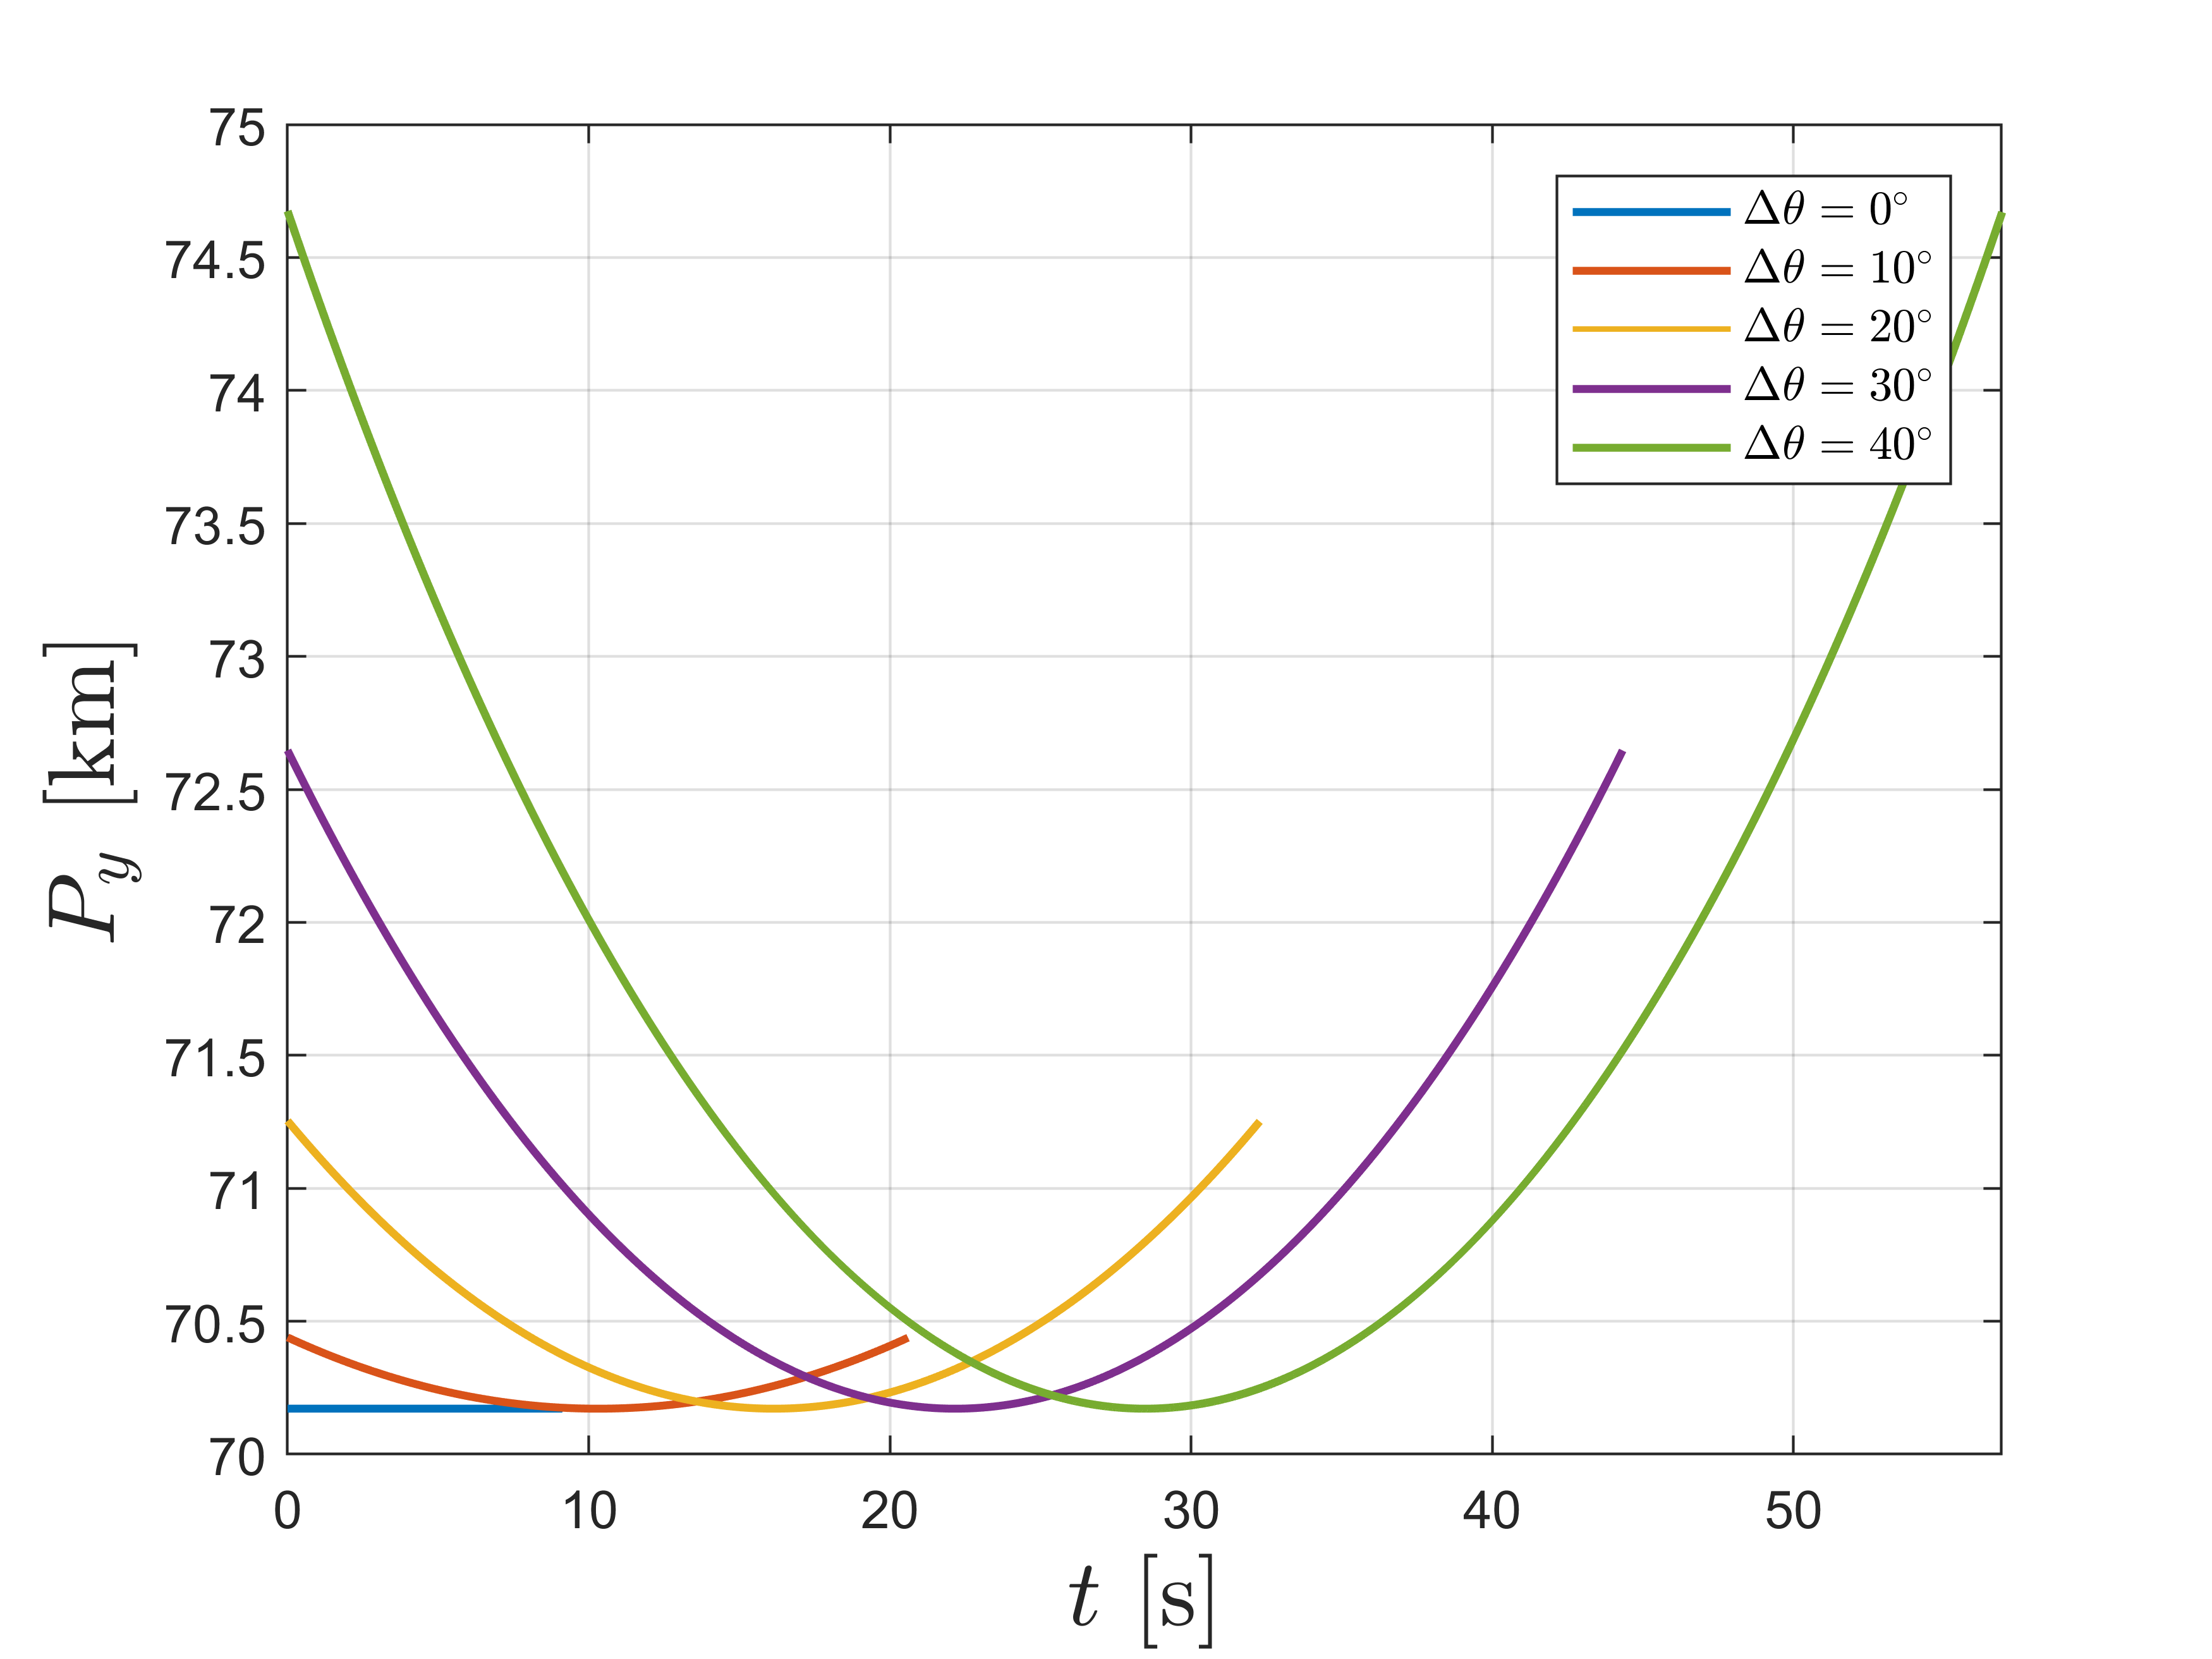
\includegraphics[width=0.45\textwidth]{figs/swath_time.png}
%   \caption{Swath width for different starting/ending pitch angles $\theta(T_0)=-\theta(T_f)$ and angular velocities $\omega_{y}$. Target track is $s_g=70 \hspace{3pt} \rm{km}$.}
% 	\label{fig:swath_time}
% \end{figure}
\begin{figure}[htbp]
  \centering
      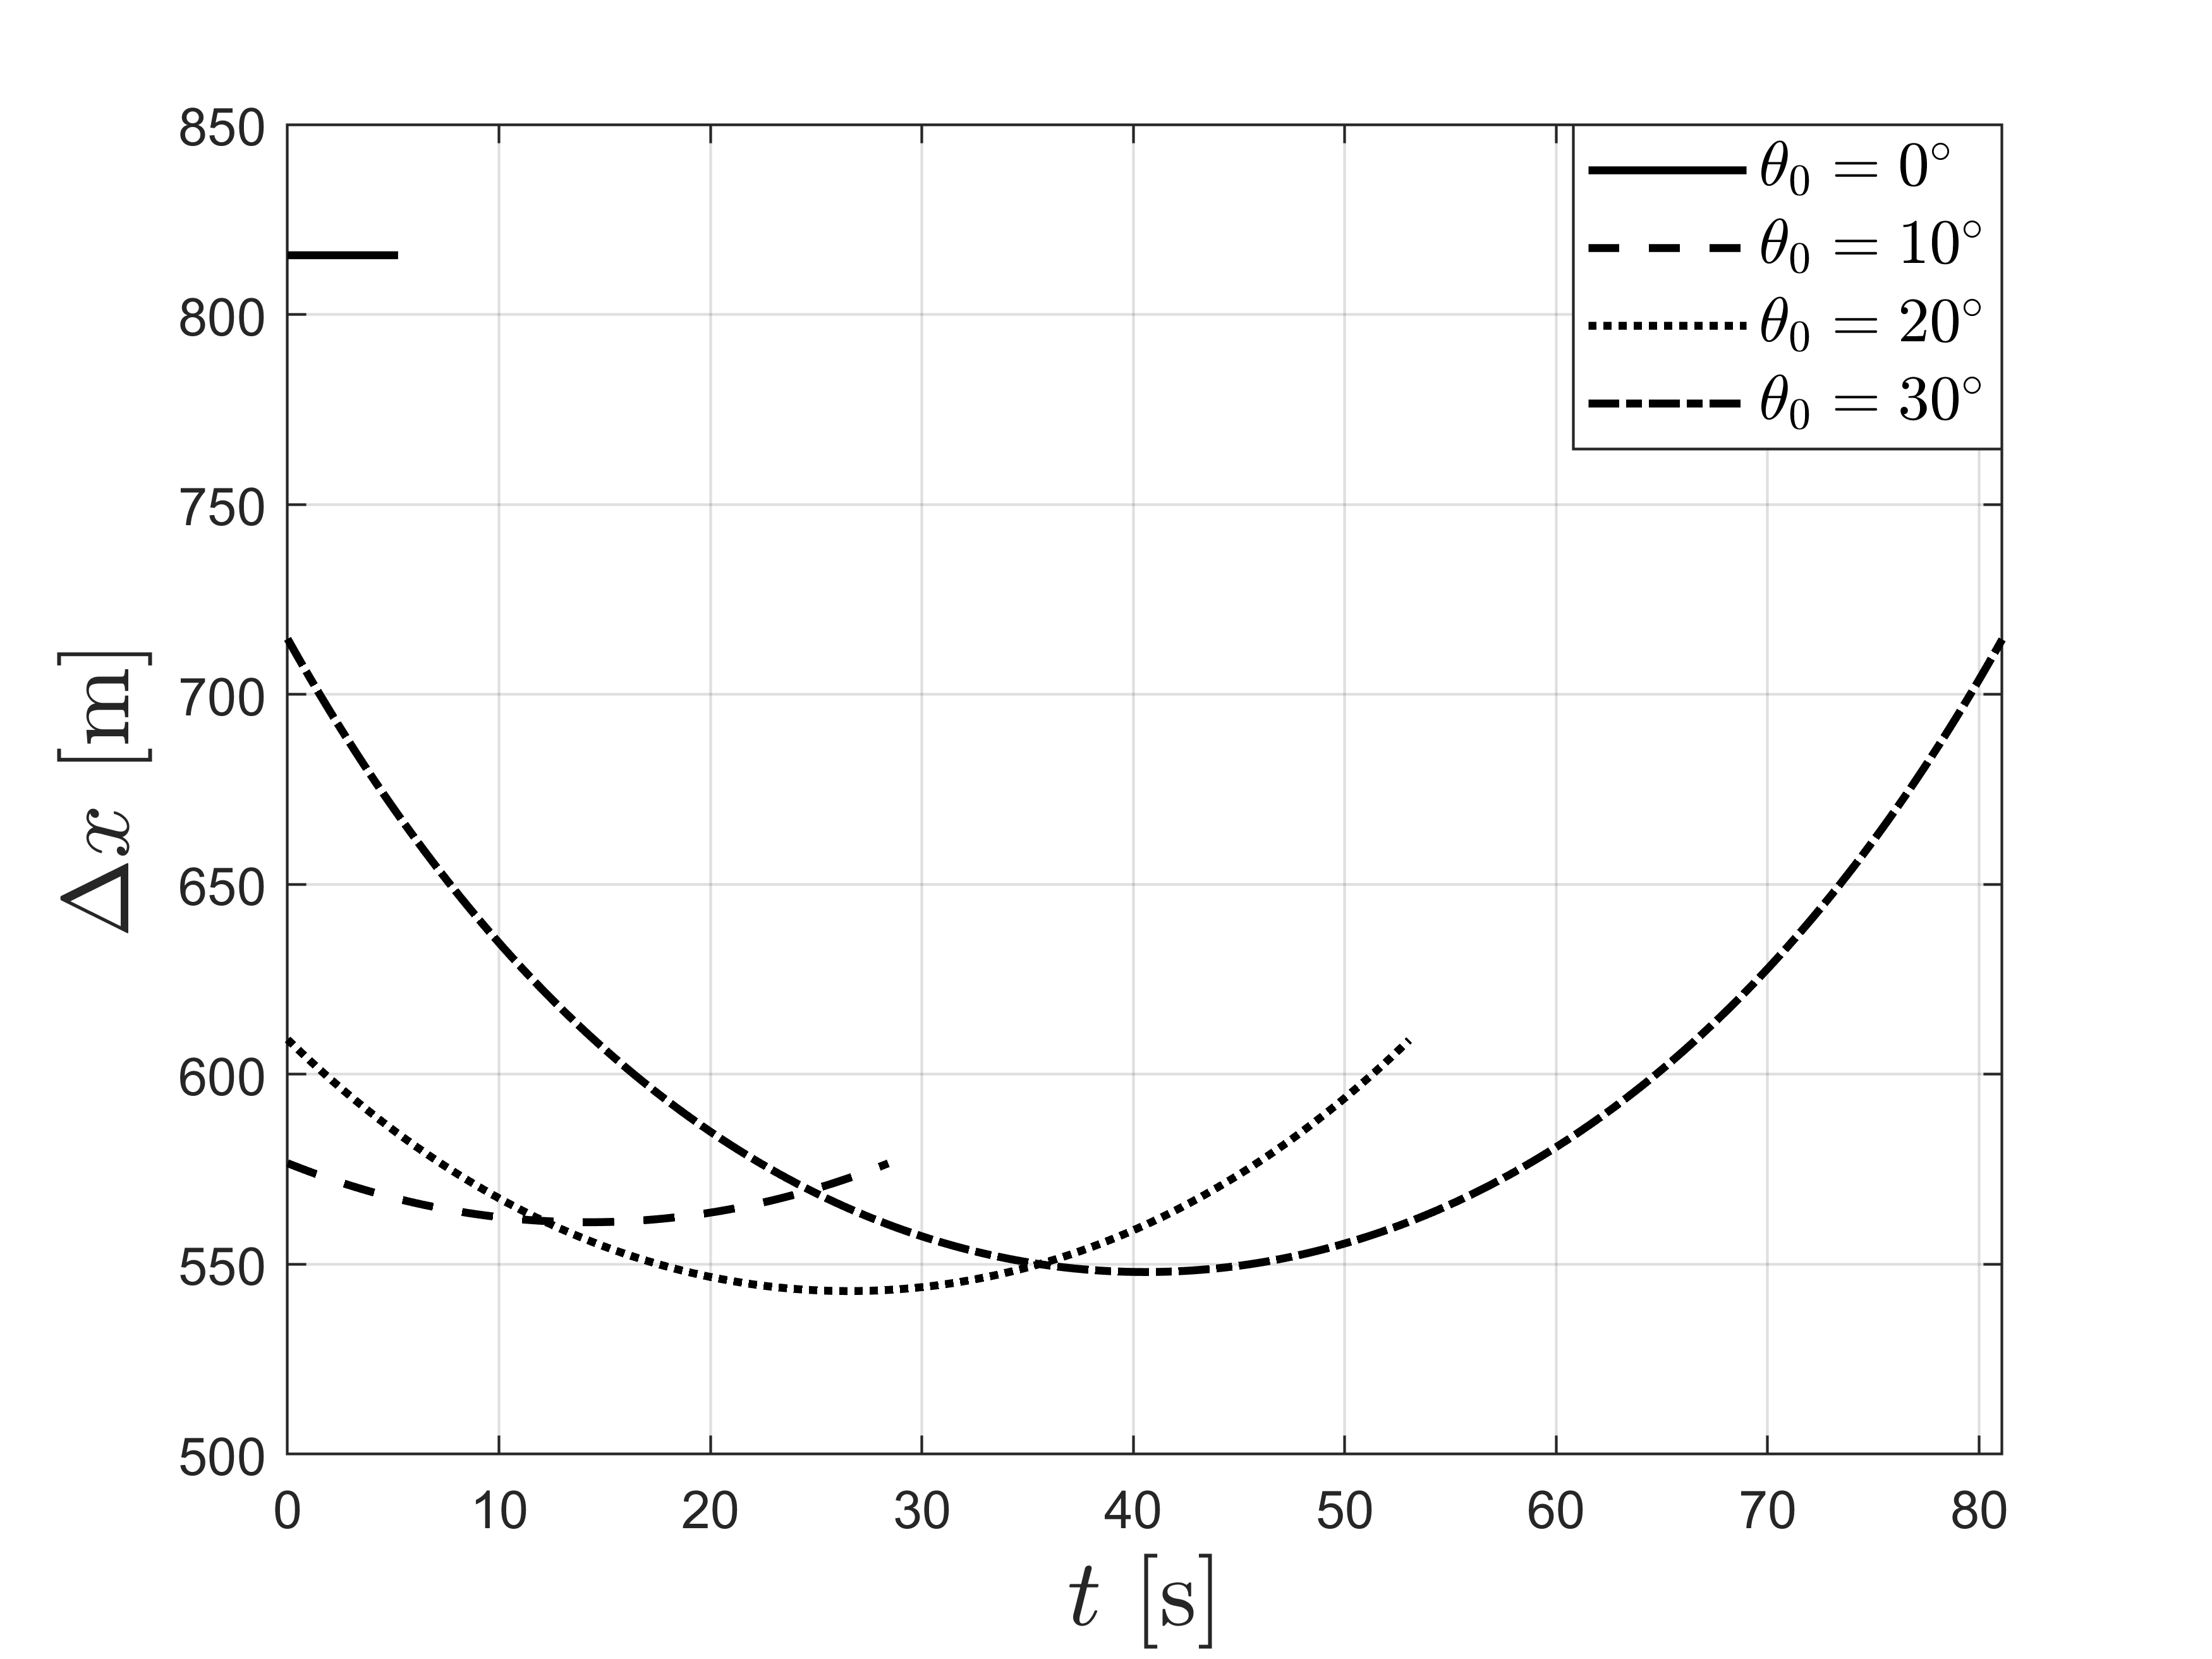
\includegraphics[width=0.48\textwidth]{figs/Delta_x.png}
  \caption{Along-track spatial resolution for different pitch angles $\theta_0=-\theta_f$ and angular velocities $\omega_{y}$.}
	\label{fig:spatial_time}
\end{figure}
\begin{figure}[htbp]
  \centering
      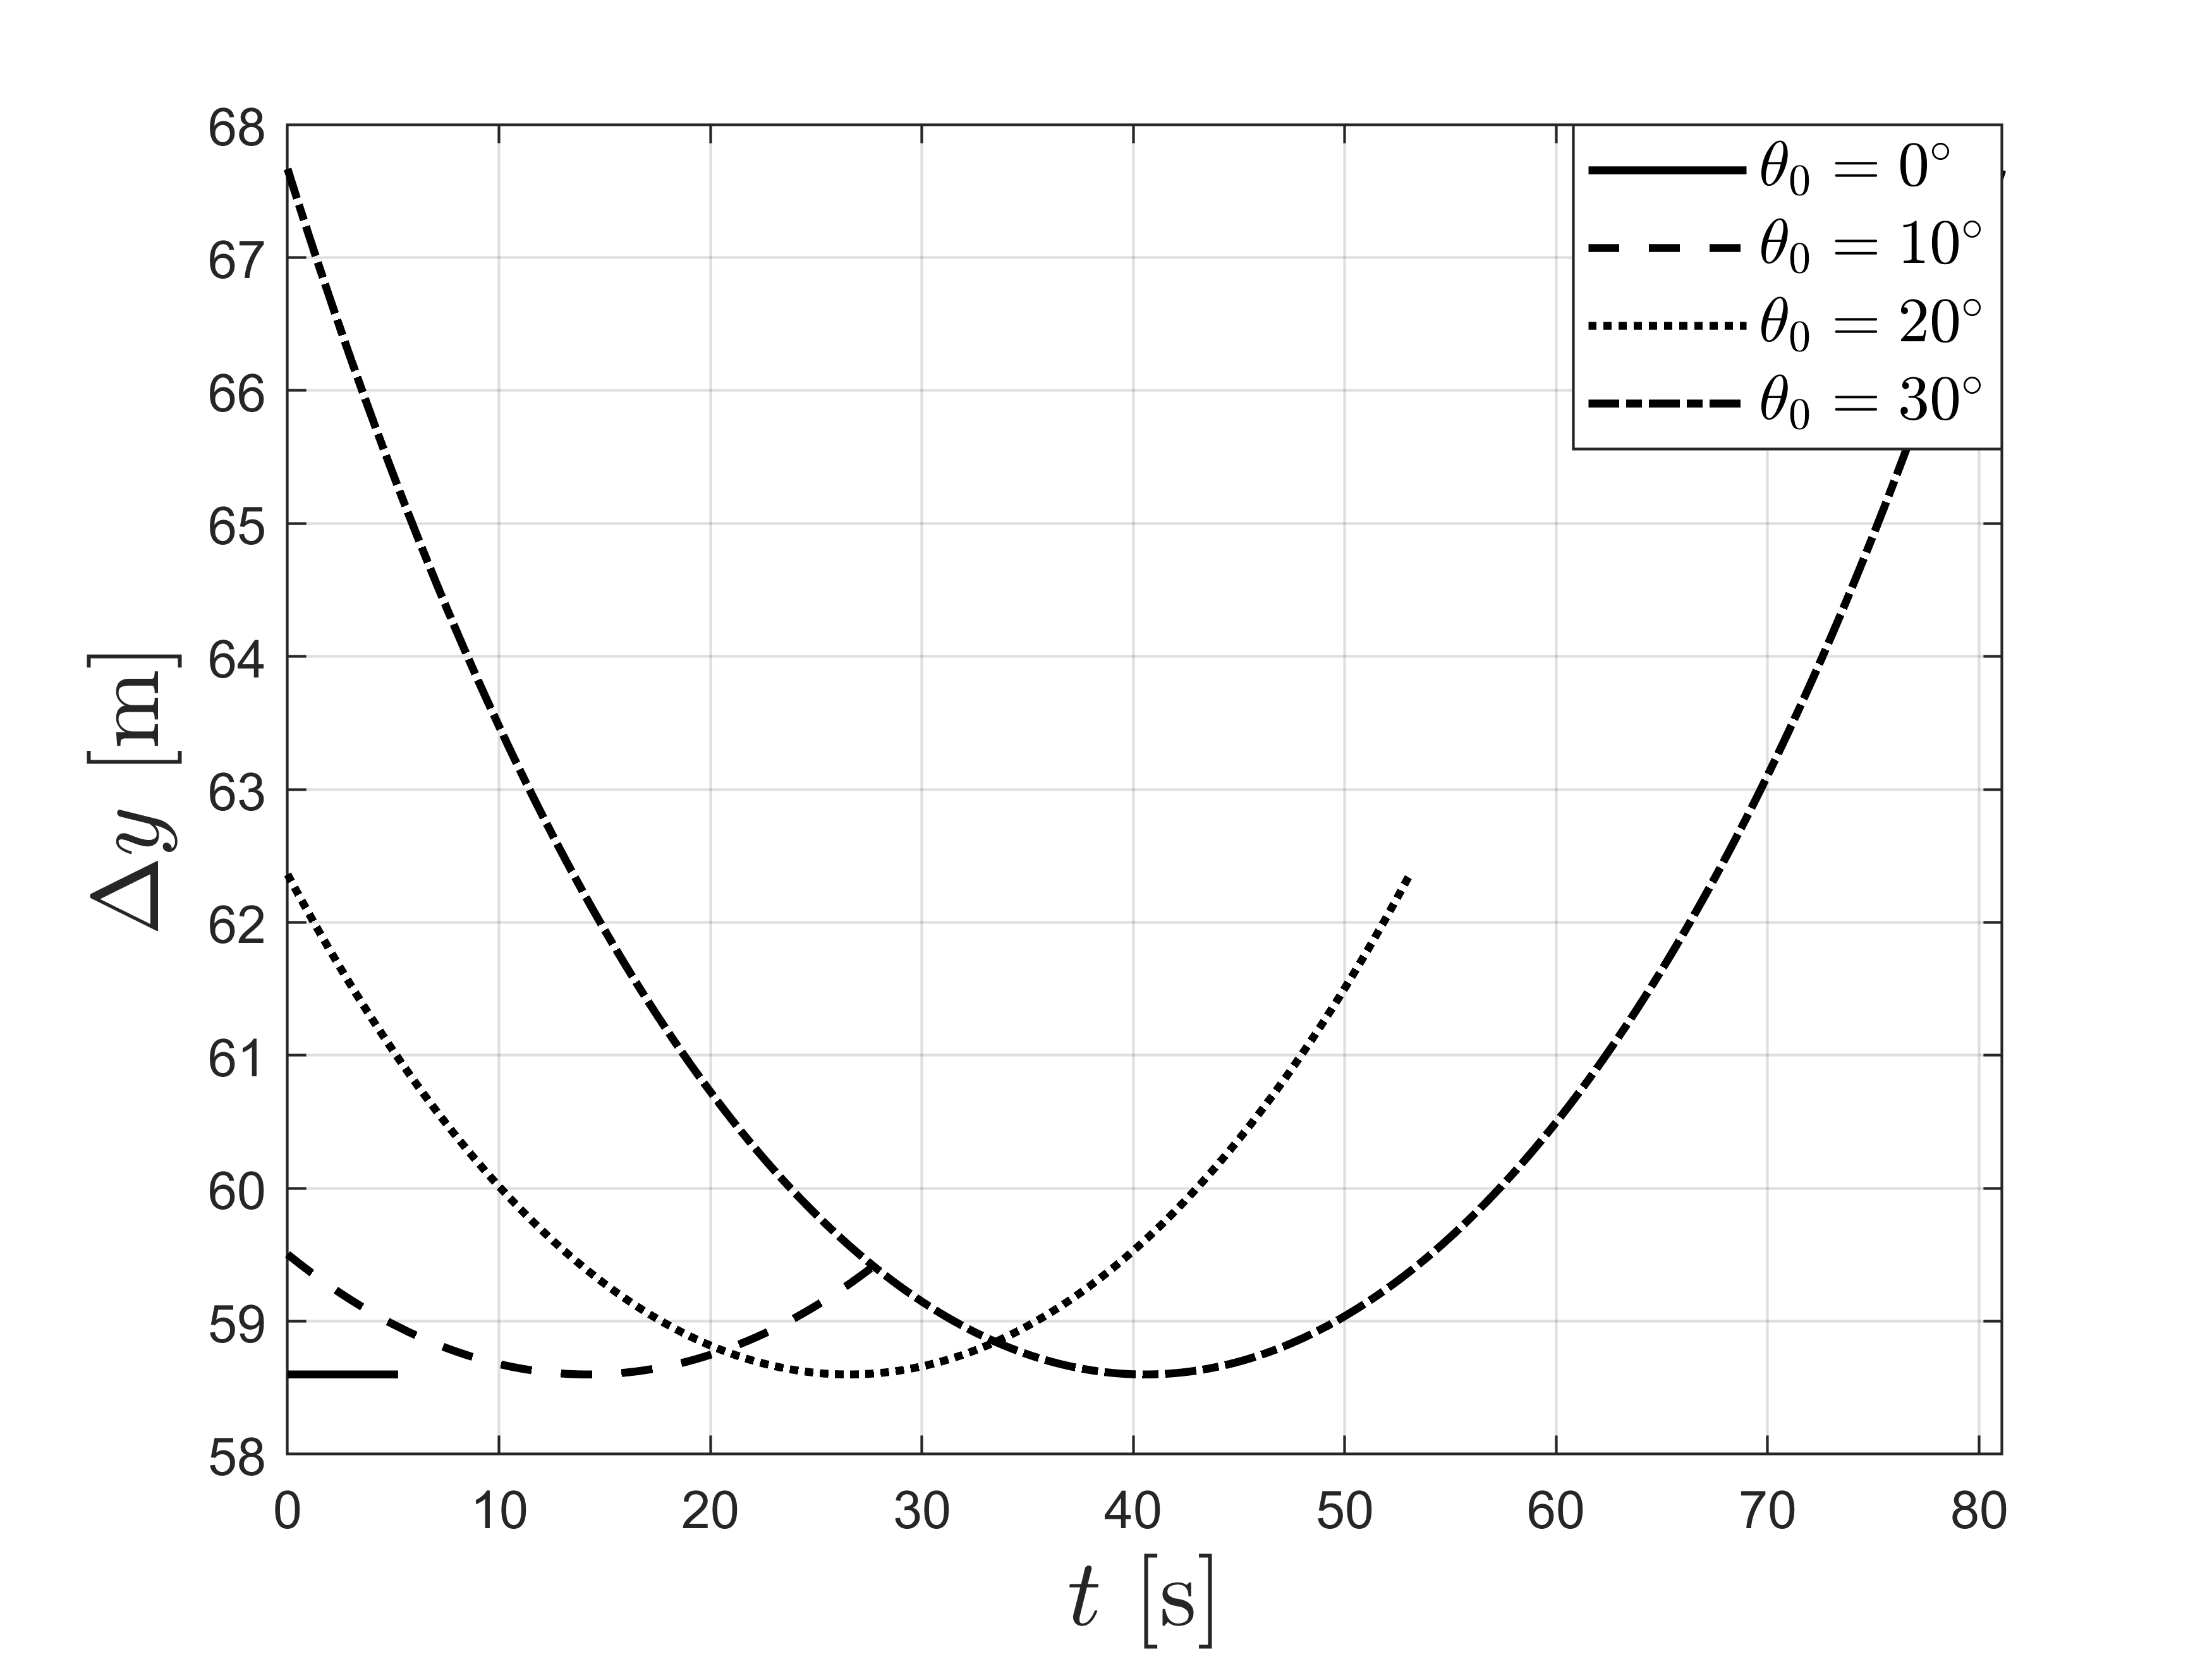
\includegraphics[width=0.48\textwidth]{figs/Delta_y.png}
  \caption{Cross-track spatial resolution for different pitch angles $\theta_0=-\theta_f$ and angular velocities $\omega_{y}$.}
	\label{fig:cross_spatial_time}
\end{figure}
% \begin{figure}[htbp]
%   \centering
%       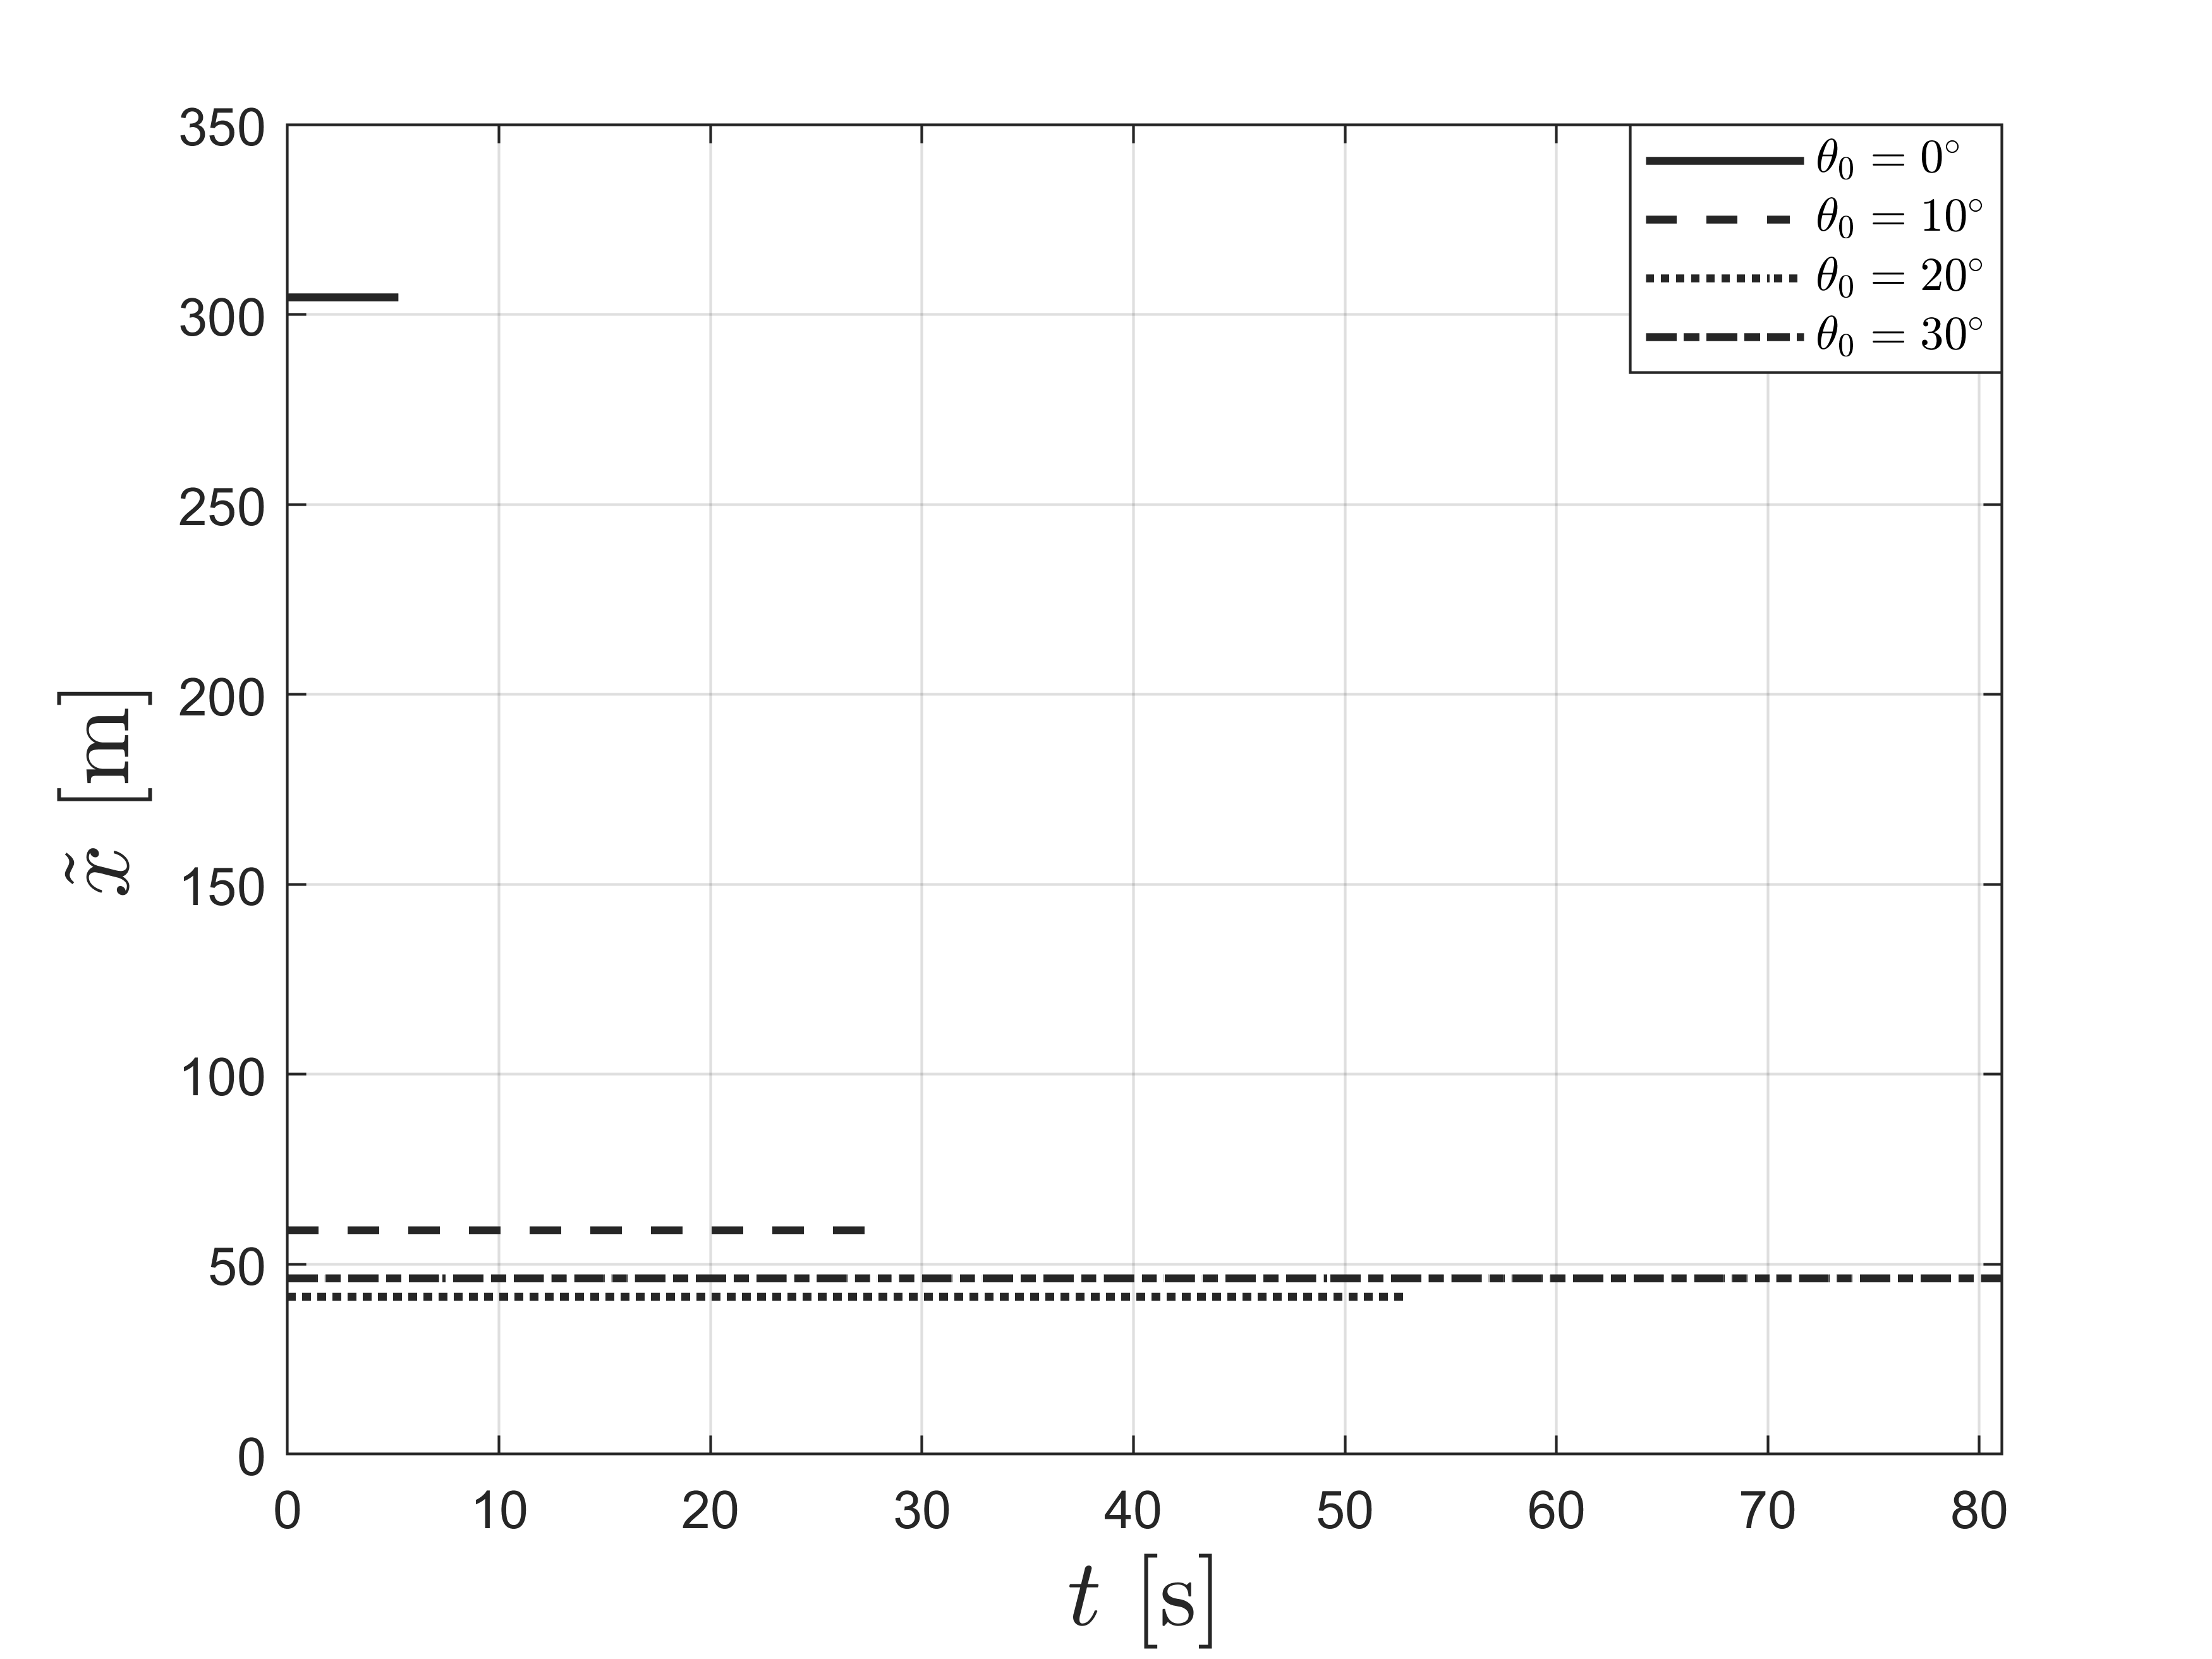
\includegraphics[width=0.48\textwidth]{figs/GSD_x.png}
%   \caption{Along-track SGSD for different starting/ending pitch angles $\theta_0=-\theta_f$ and angular velocities $\omega_{y}$. Target track is $s_g=42.41 \hspace{3pt} \rm{km}$.\hl{tabulate}}
% 	\label{fig:GSDx}
% \end{figure}
\begin{table}[htbp]
	\caption{Along-track SGSD}
	\label{tab:SGSD}
	\centering
			\begin{tabular}{l l l| l}
				\hline
				$\theta_0$ [$^{\circ}$] & $\omega_y$ [$^{\circ}\rm{/s}$] & $\Delta T$ [$\rm{s}$]&  $\tilde{x}$ [$\rm{m}$] \\
				\hline
				0 & 0 & 5.23 & 346  \\
				10 & -0.704 & 28.41 & 66.96 \\
				20 & -0.754 & 53.05 & 47.09 \\
				30 & -0.740 & 81.09 & 52.59 \\
				\hline
				\end{tabular}
\end{table}
\begin{figure}[htbp]
  \centering
      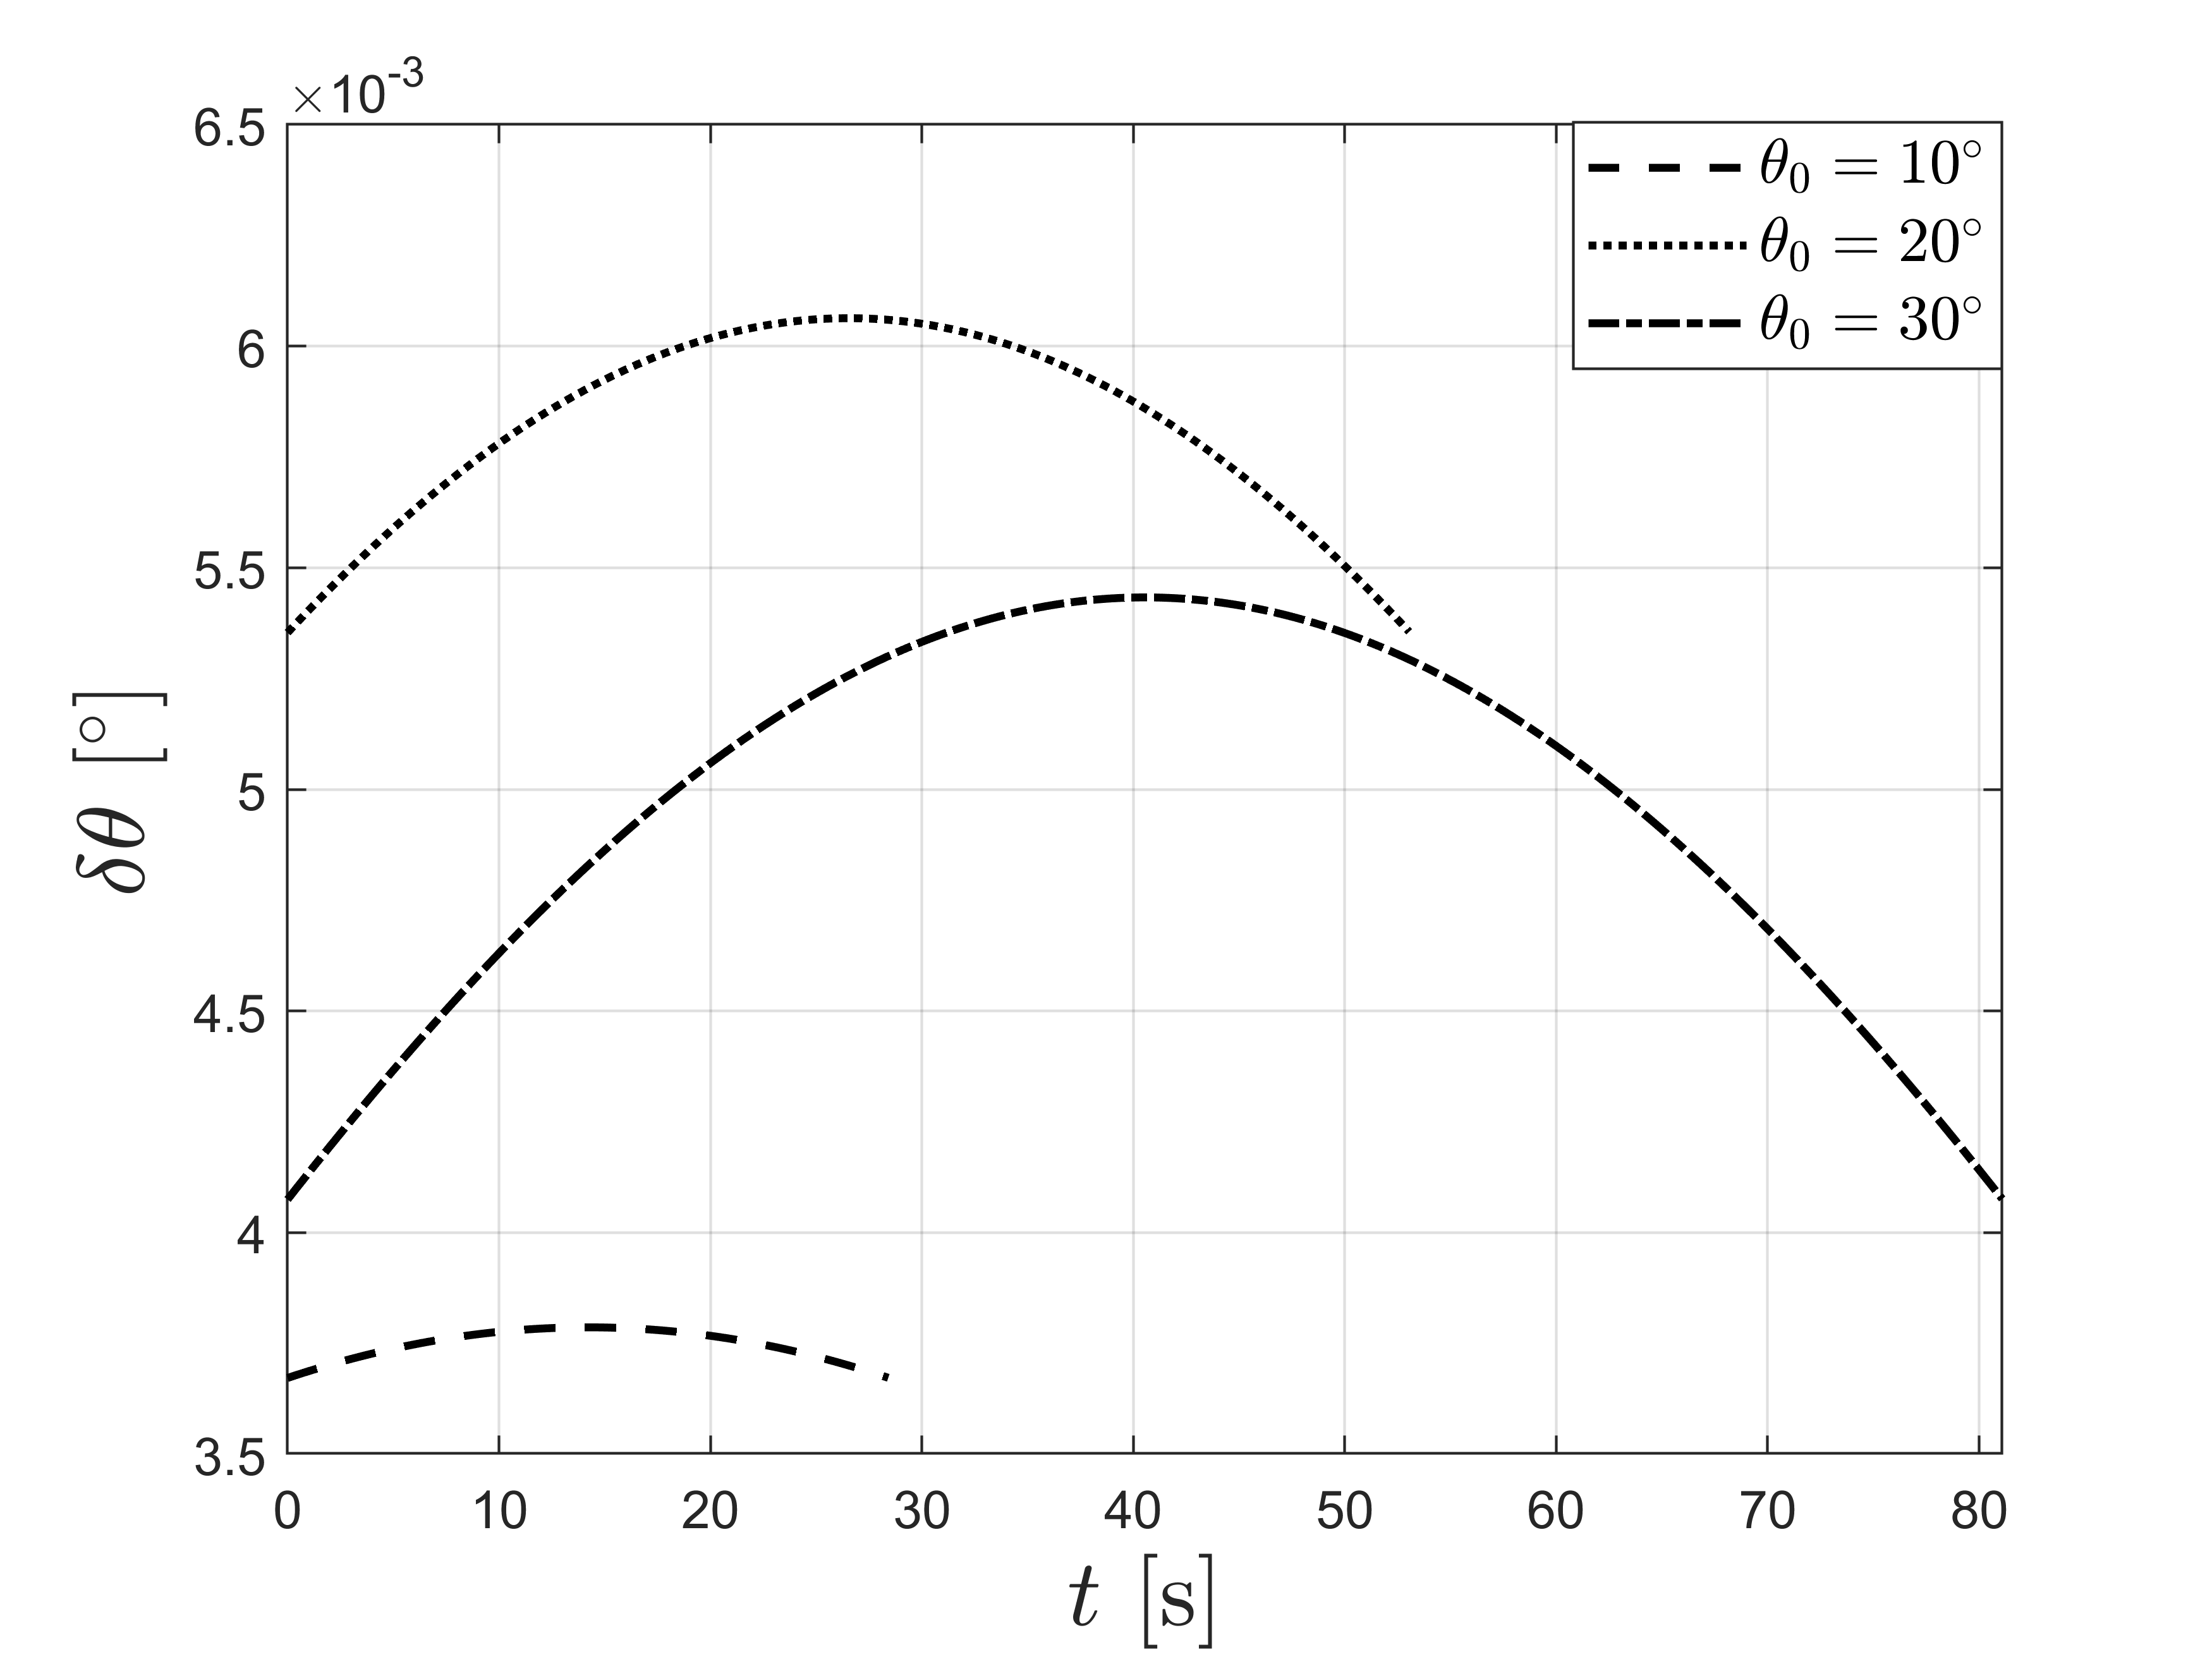
\includegraphics[width=0.48\textwidth]{figs/dtheta.png}
  \caption{Required pitch accuracy throughout the slew maneuvers for different $\theta_0$.}
	\label{fig:dtheta}
\end{figure}
% \begin{figure}[htbp]
%   \centering
%       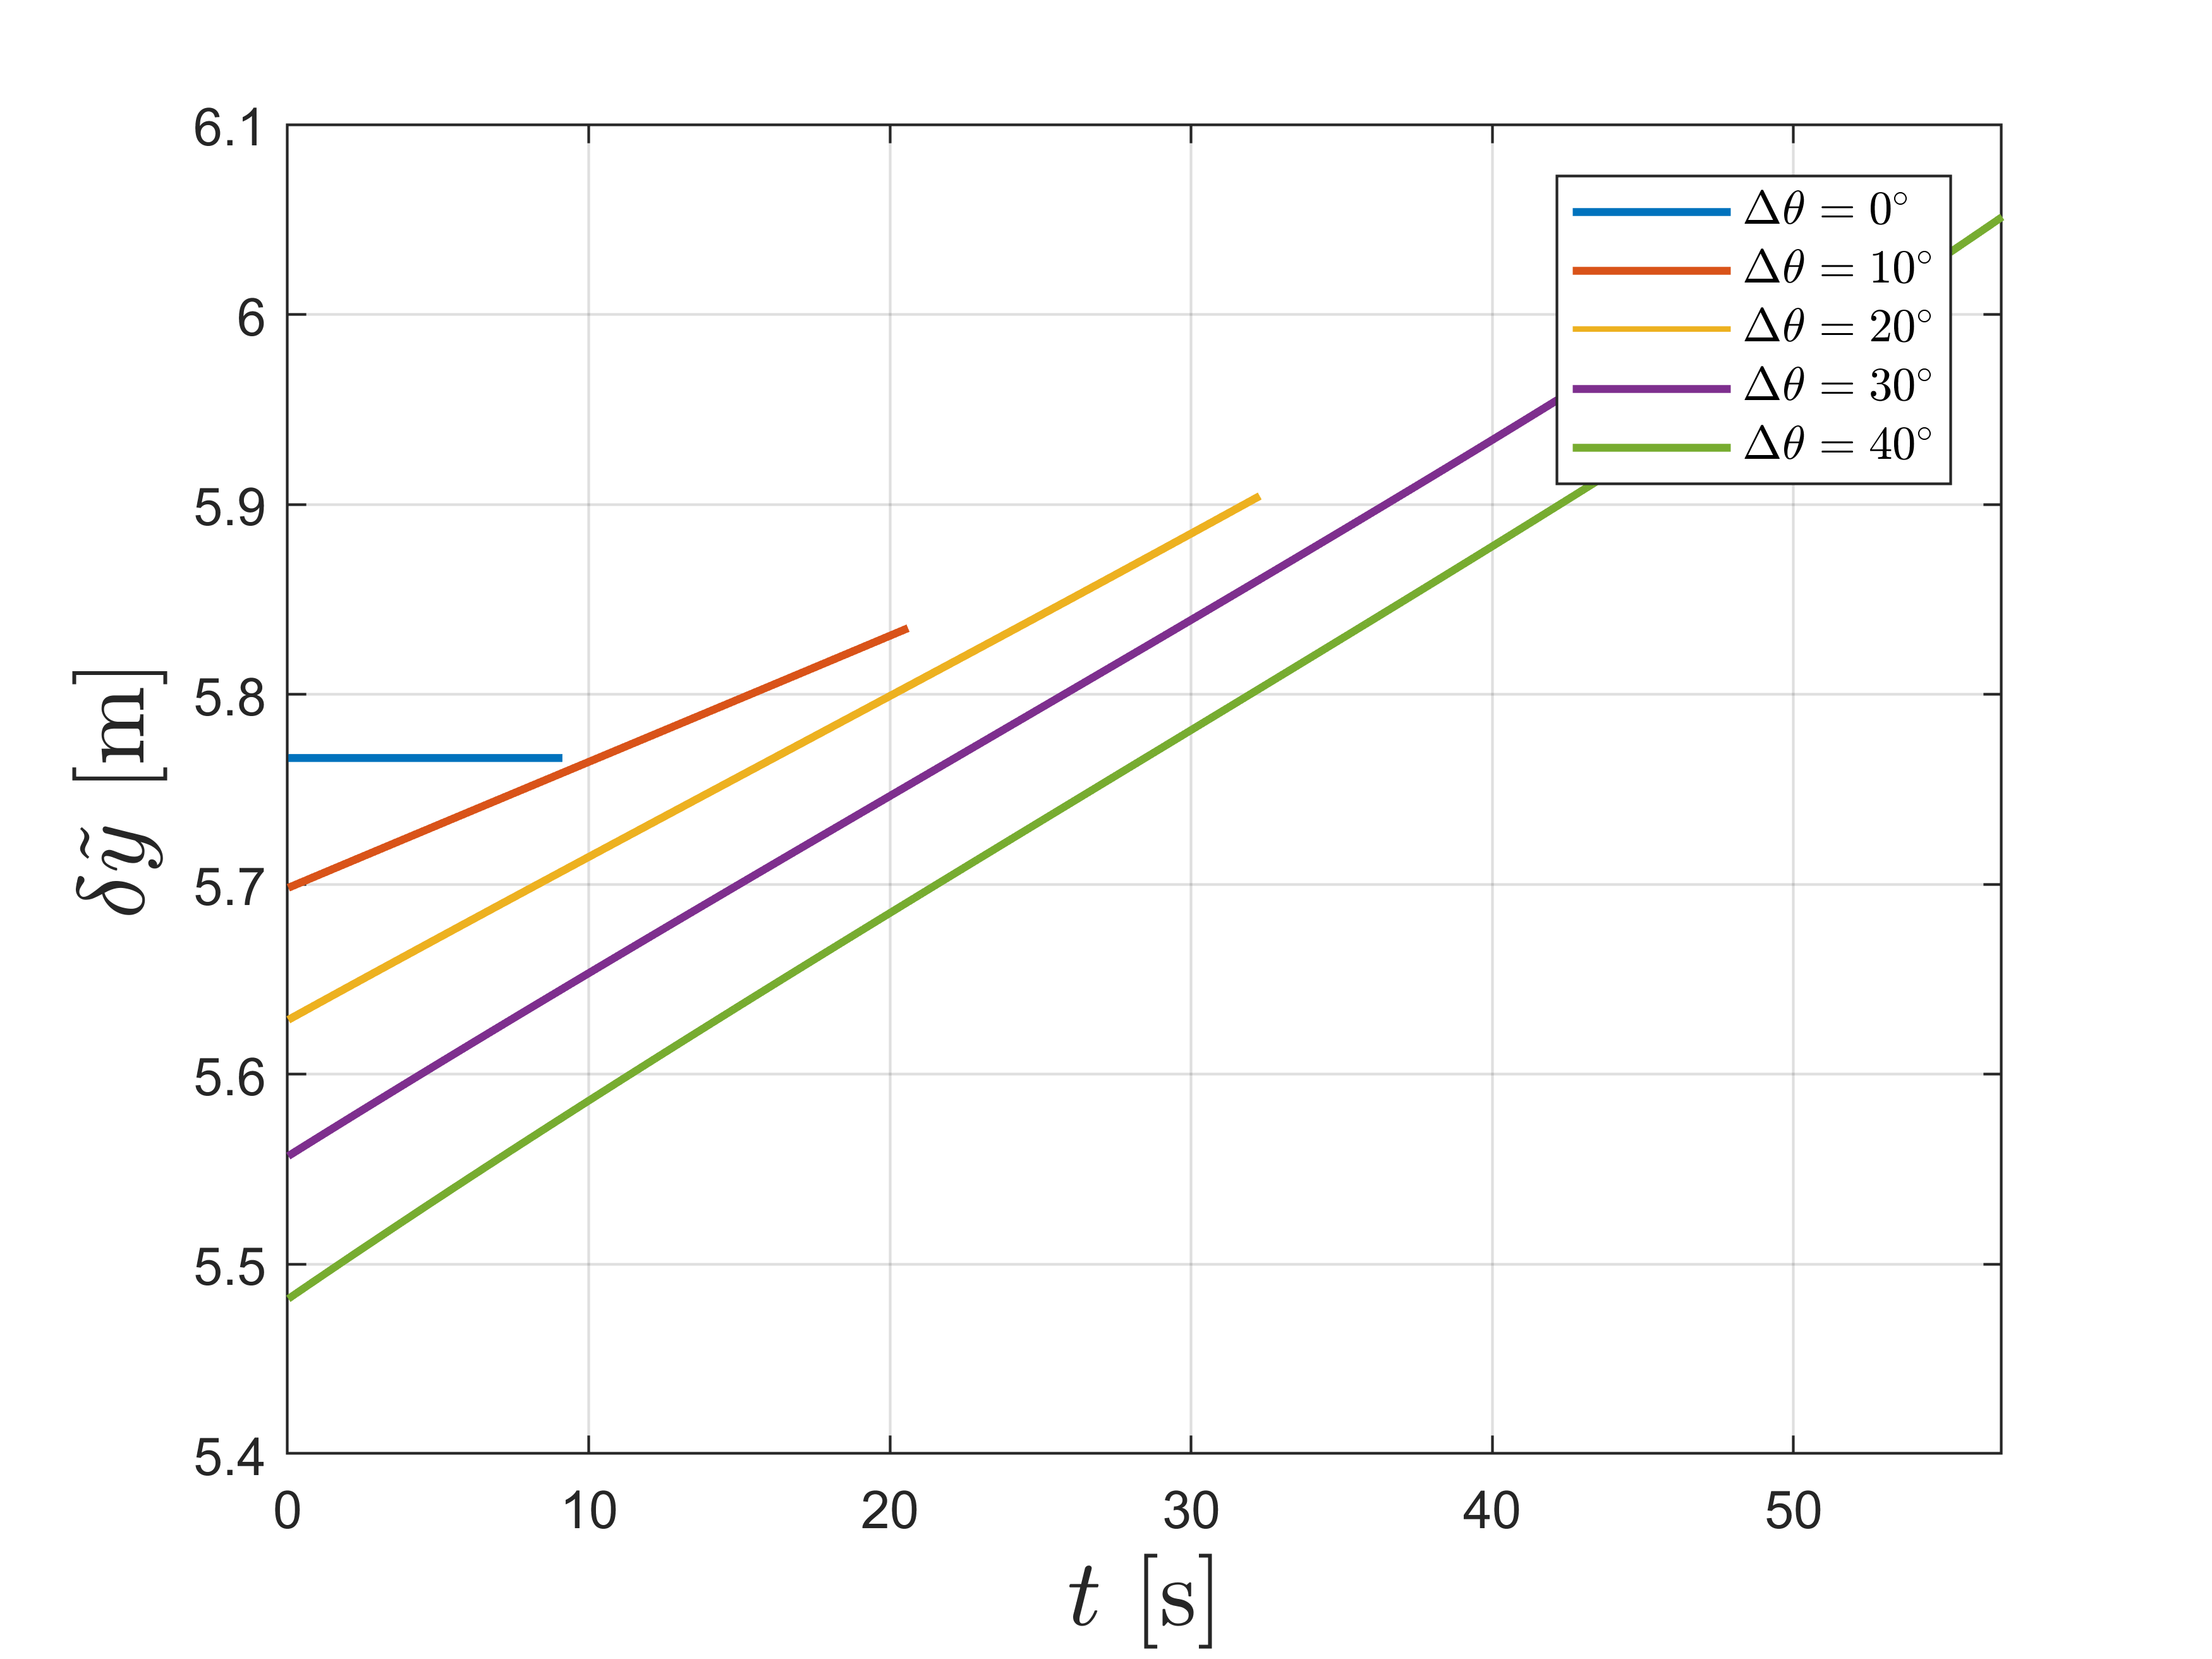
\includegraphics[width=0.45\textwidth]{figs/GSD_y.png}
%   \caption{Cross-track RGS for different starting/ending pitch angles $\theta(t_0)=-\theta(t_f)$ and angular velocities $\omega_{y}$. Target track is $s_g=70 \hspace{3pt} \rm{km}$.}
% 	\label{fig:GSDy}
% \end{figure}
% \begin{figure}[htbp]
%   \centering
%       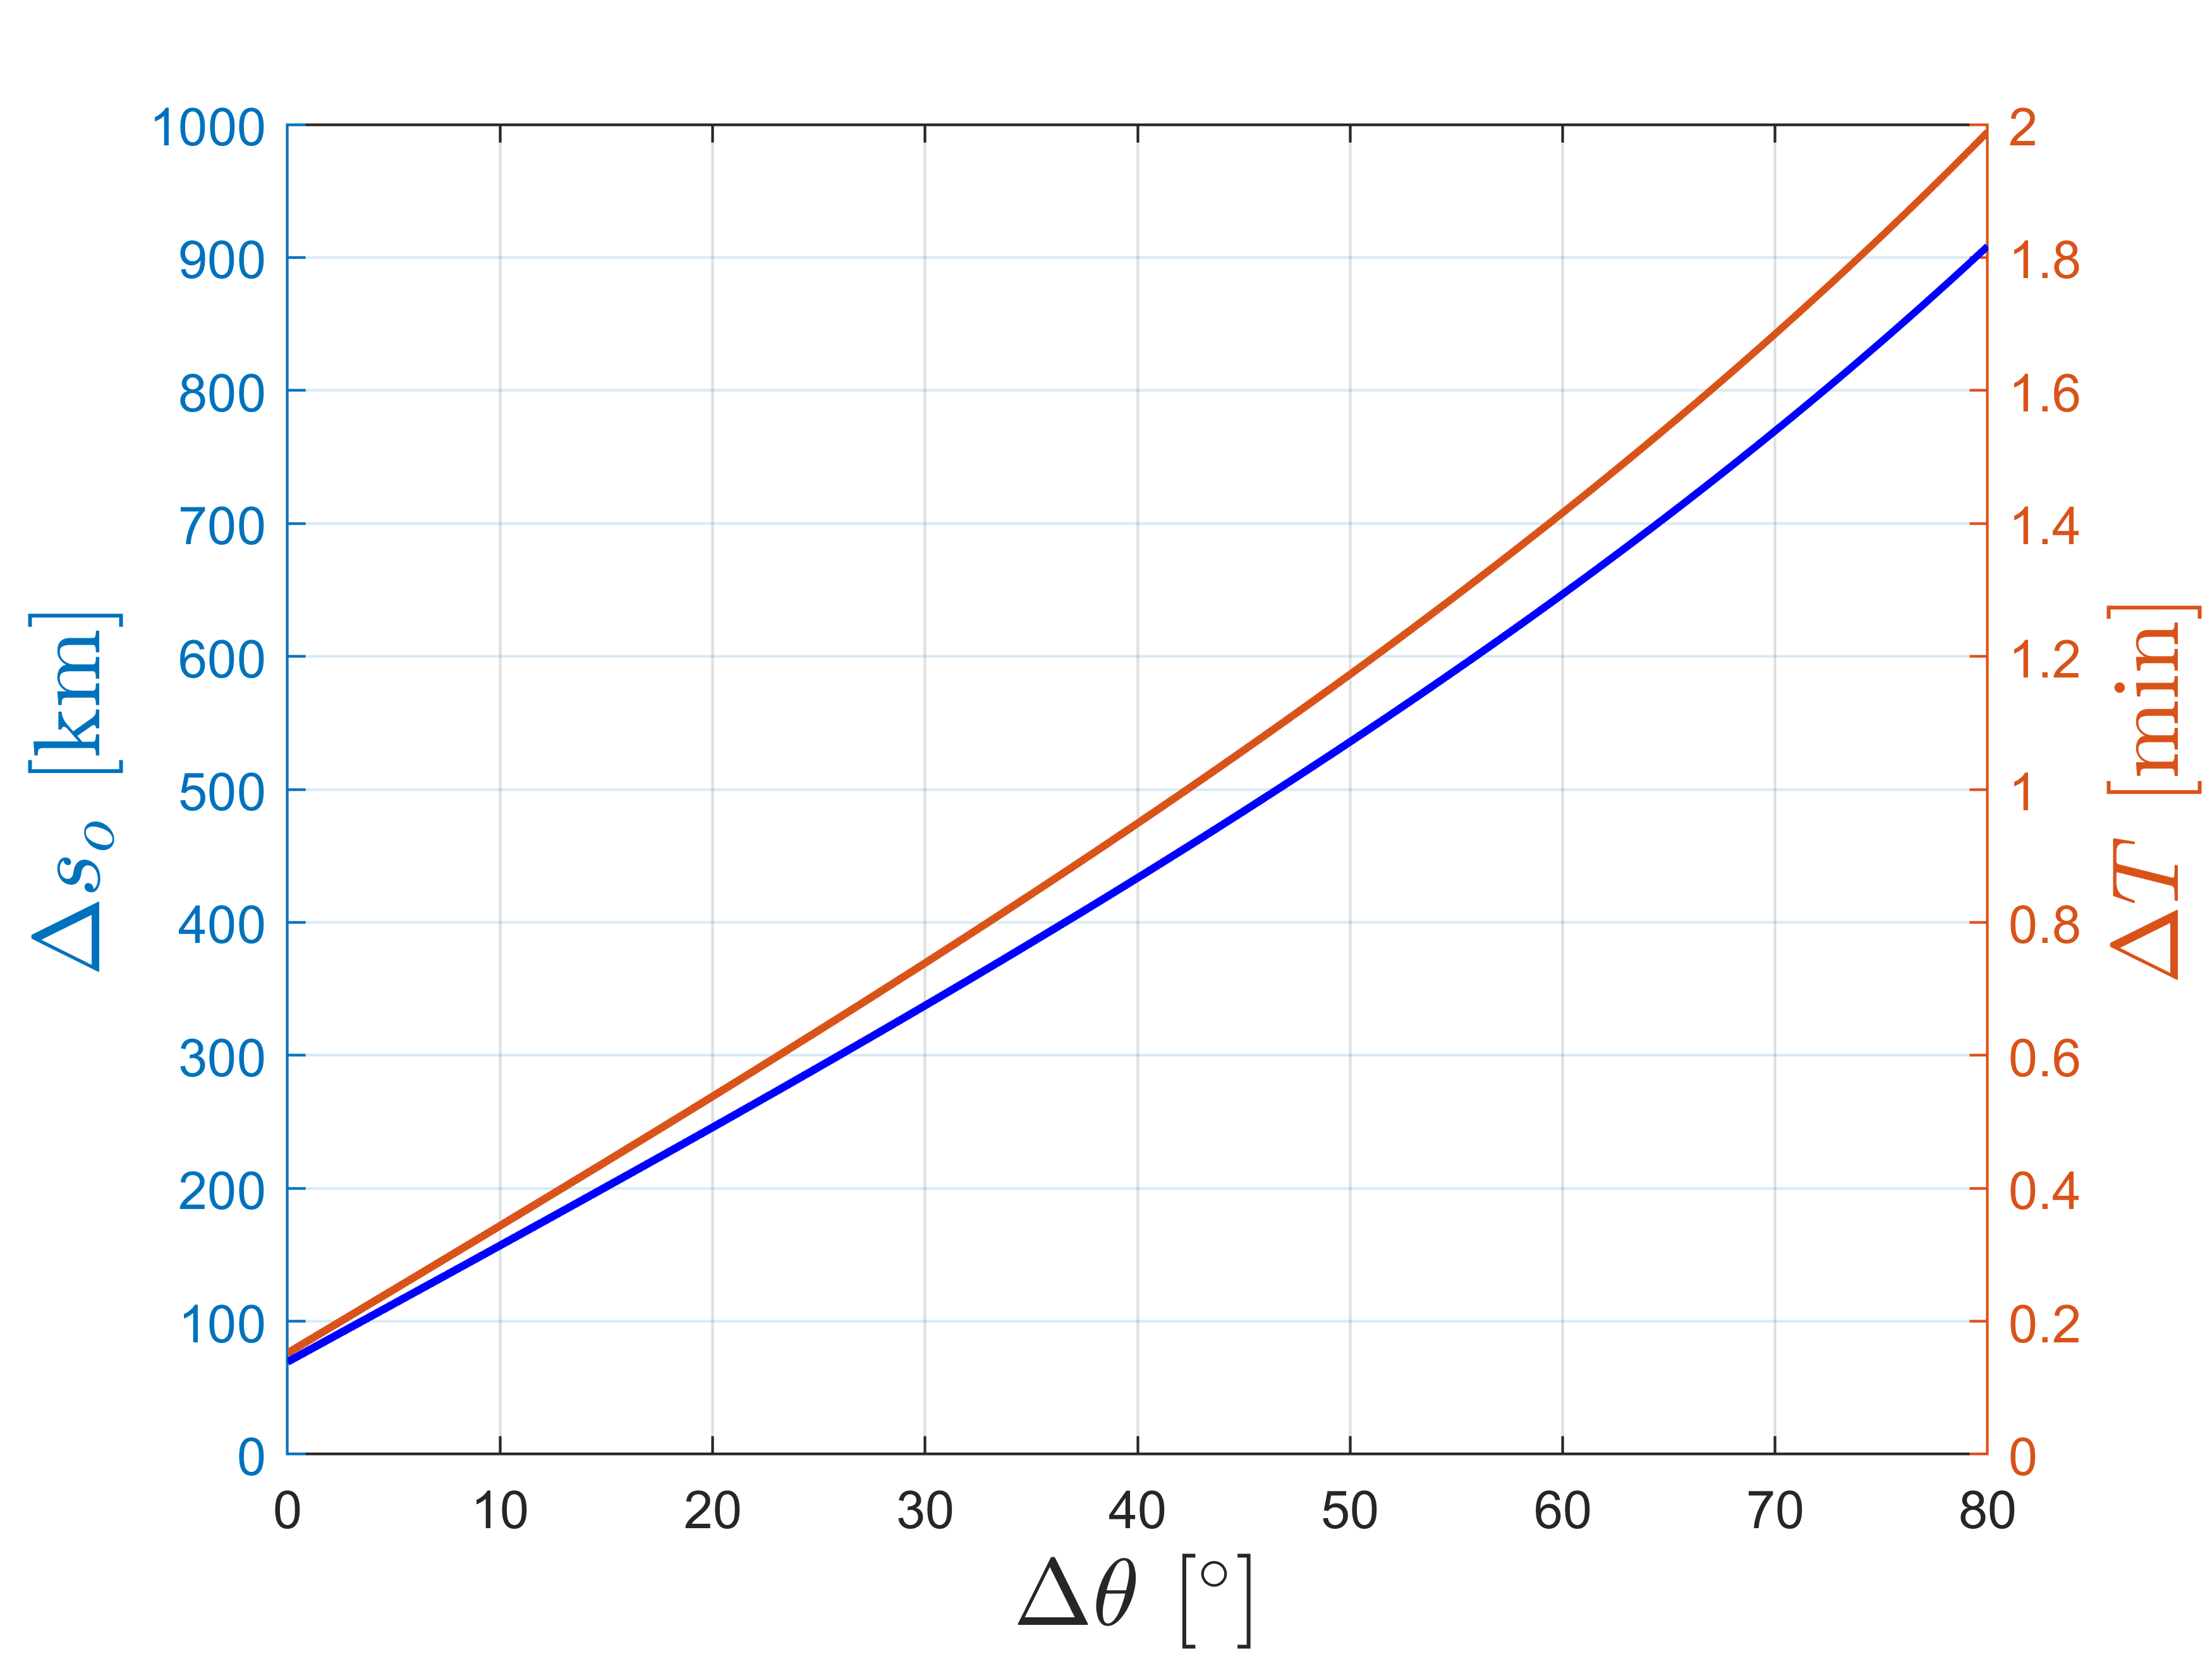
\includegraphics[width=0.45\textwidth]{figs/track_time.png}
%   \caption{In-orbit track distance and observation time vs. starting/ending pitch angles $\theta(T_0)=-\theta(T_f)$ and angular velocities $\omega_{y}$. Target track is $s_g=70 \hspace{3pt} \rm{km}$.}
% 	\label{fig:track_time}
% \end{figure}
% \subsubsection{In-track Slew Maneuver with Perturbations}
% Figures \ref{fig:spatial_time_err} and \ref{fig:GSD_x_err} show how noise in the satellite system causes deviations to the sensor output performance and the nominal reference ground track. Noise is assumed to be Gaussian-distributed with zero mean such that noise due to the spacecraft structure and the actuators (e.g. reaction wheels) is represented with $\delta\boldsymbol{\omega} \sim \mathcal{N}(0, 0.1^{\circ}/\rm{s})$. 
% Table \ref{tab:statistics} shows the statistics for spatial resolution, GSD and pitch angle due to variations in vehicle angular velocity $\boldsymbol{\omega}$. 
% \begin{figure}[htbp]
%   \centering
%       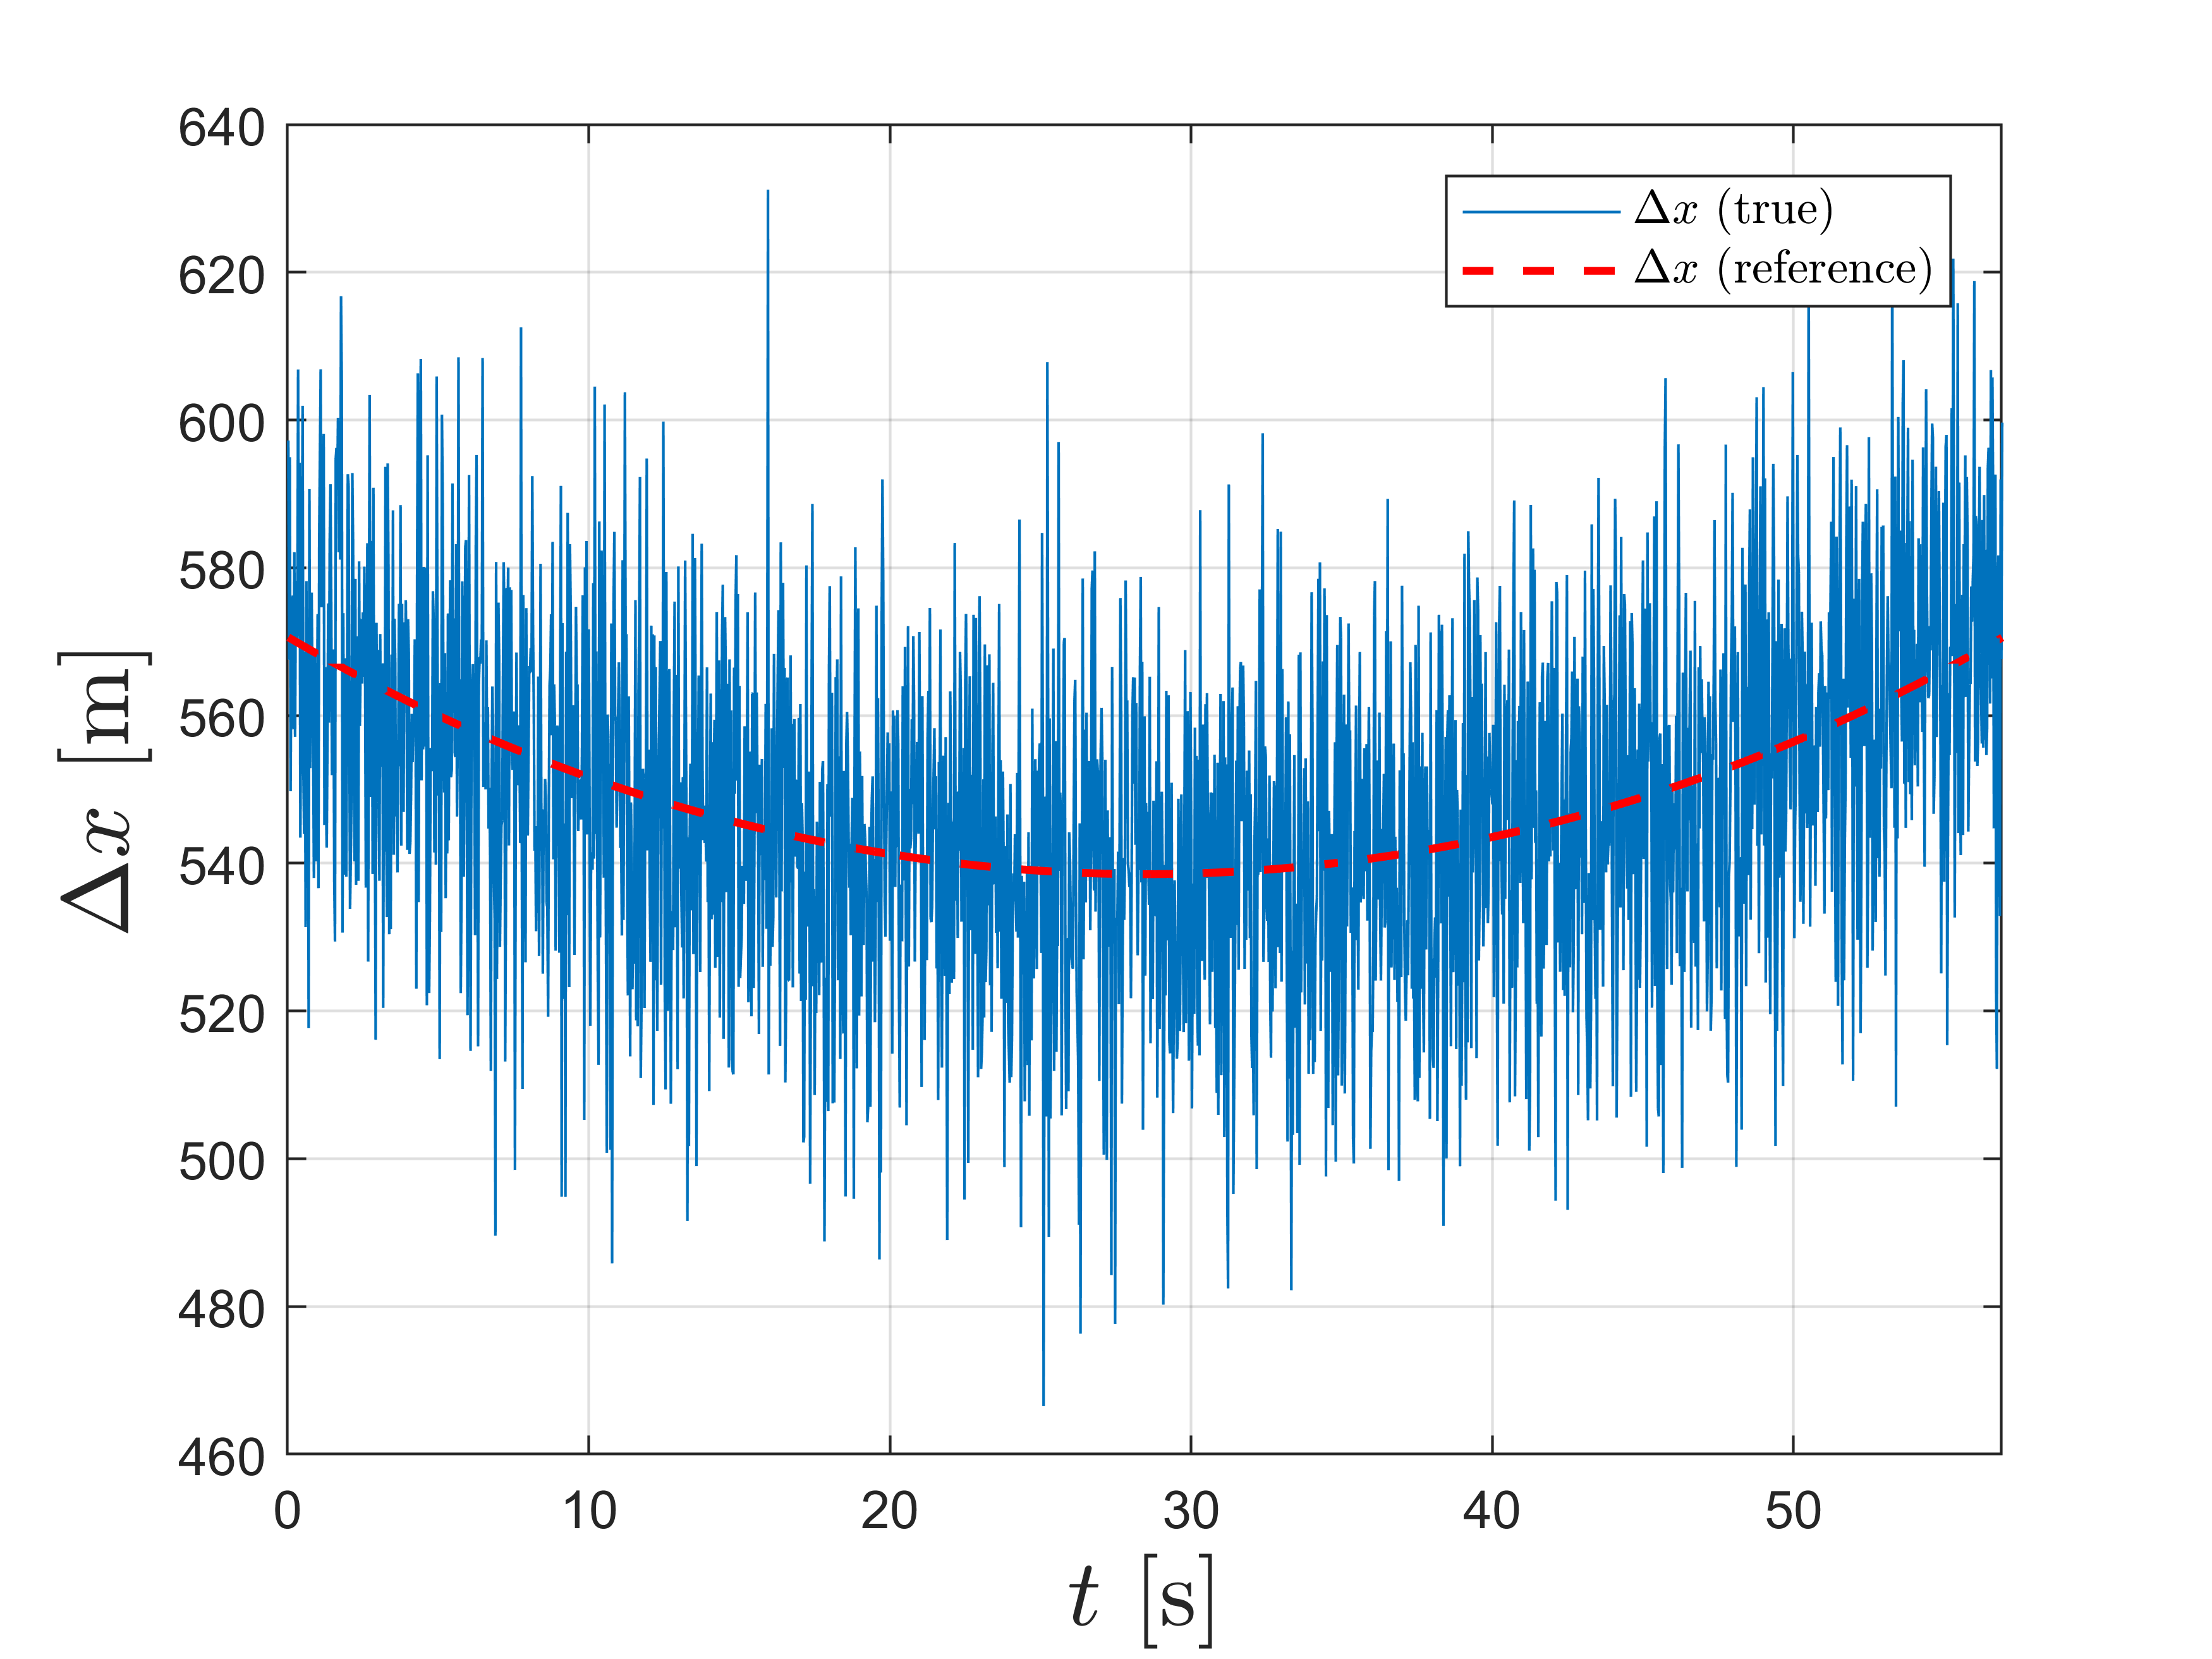
\includegraphics[width=0.45\textwidth]{figs/spatial_time_err.png}
%   \caption{In-track spatial resolution for $\Delta \theta = 40^{\circ}$, $\omega_{y}=-0.7025^{\circ}/\rm{s}$ and $\delta\boldsymbol{\omega} \sim \mathcal{N}(0, 0.1^{\circ}/\rm{s})$.}
% 	\label{fig:spatial_time_err}
% \end{figure}
% \begin{figure}[htbp]
%   \centering
%       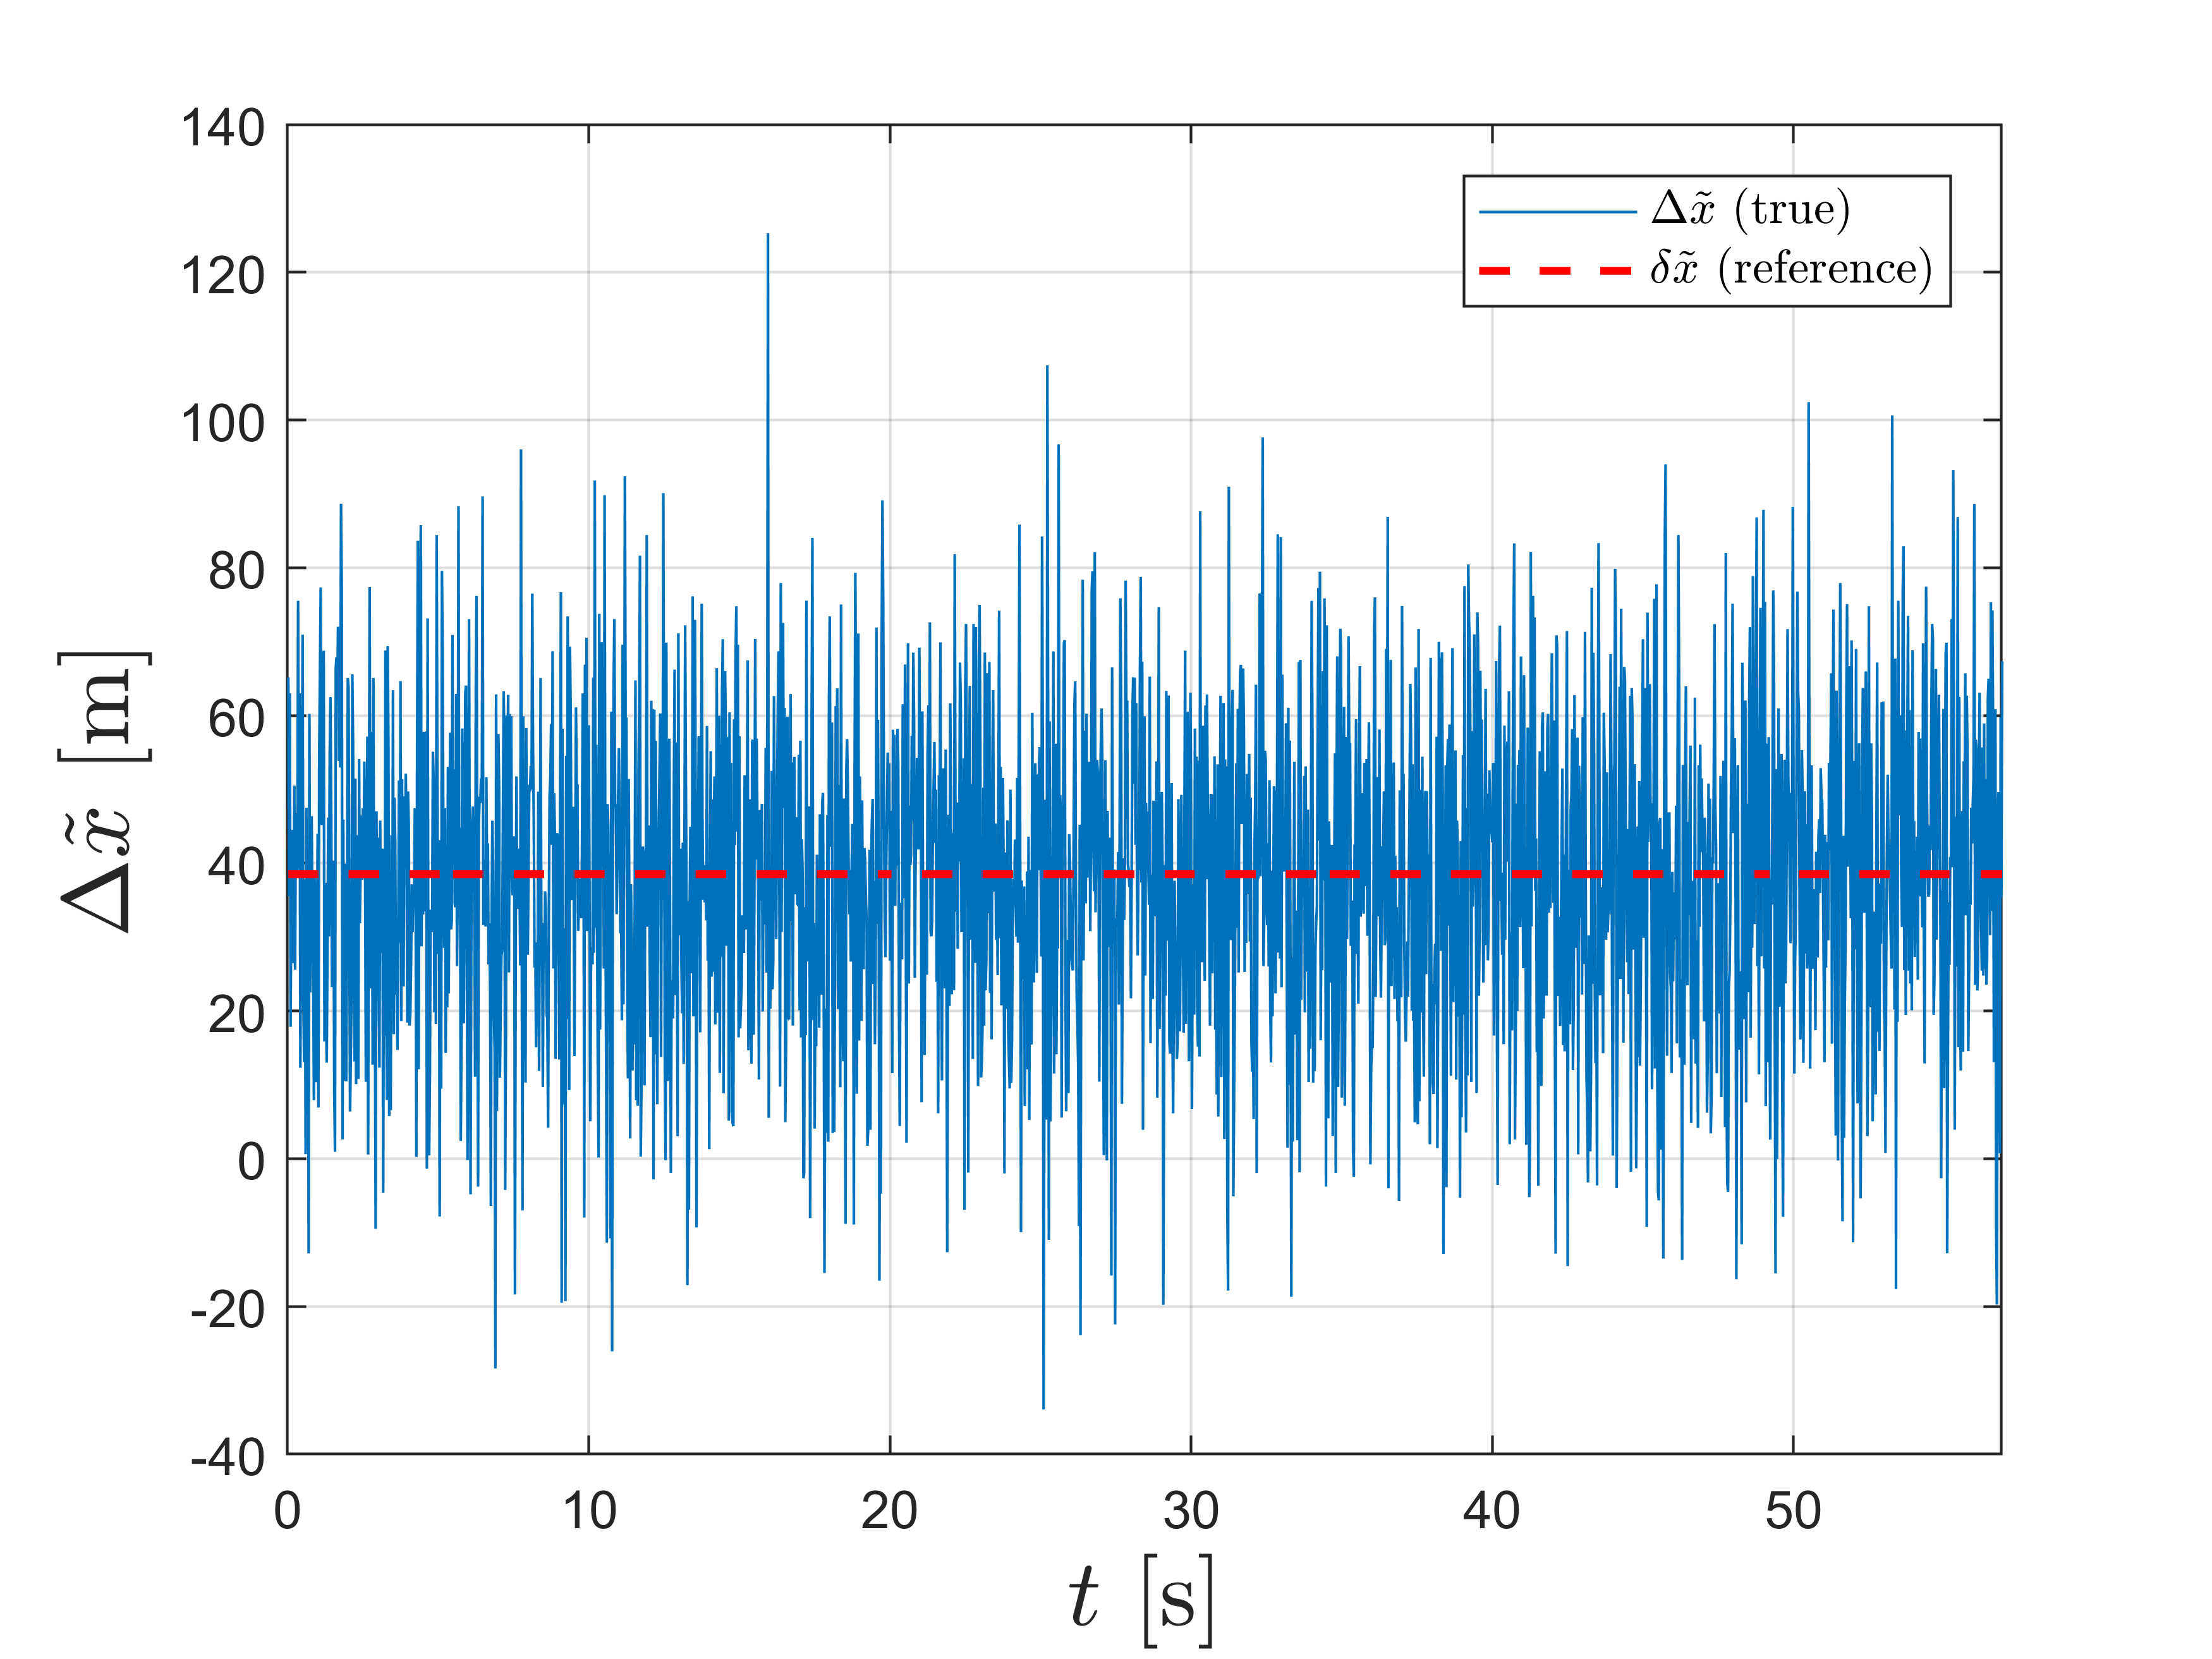
\includegraphics[width=0.45\textwidth]{figs/GSD_x_err.png}
%   \caption{In-track GSD for $\Delta \theta = 40^{\circ}$, $\omega_{y}=-0.7025^{\circ}/\rm{s}$ and $\delta\boldsymbol{\omega} \sim \mathcal{N}(0, 0.1^{\circ}/\rm{s})$.}
% 	\label{fig:GSD_x_err}
% \end{figure}
% \begin{table}[htbp]
% 	\caption{Statistics for satellite spatial imaging performance during slew maneuver}
% 	\label{tab:statistics}
% 	\centering
% 			\begin{tabular}{l r r r r}
% 				\hline
% 				Value & Mean & Standard Deviation & Maximum & Minimum \\
% 				$\Delta x$ & $549.19 \hspace{3pt} \rm{m}$ & $23.84 \hspace{3pt} \rm{m}$ & $632.46 \hspace{3pt} \rm{m}$ & $442.43 \hspace{3pt} \rm{m}$ \\
% 				$\Delta y$ & $64.28 \hspace{3pt} \rm{m}$ & $21.62 \hspace{3pt} \rm{m}$ & $141.00 \hspace{3pt} \rm{m}$ & $-9.84 \hspace{3pt} \rm{m}$ \\
% 				$P_{y}$ & $71.64 \hspace{3pt} \rm{km}$ & $1.33 \hspace{3pt} \rm{km}$ & $74.71 \hspace{3pt} \rm{km}$ & $70.17 \hspace{3pt} \rm{km}$ \\
% 				$\delta x$ & $510.48 \hspace{3pt} \rm{m}$ & $9.51 \hspace{3pt} \rm{m}$ & $532.37 \hspace{3pt} \rm{m}$ & $500.00 \hspace{3pt} \rm{m}$ \\
% 				$\tilde{x}$ & $38.71 \hspace{3pt} \rm{m}$ & $21.86 \hspace{3pt} \rm{m}$ & $102.60 \hspace{3pt} \rm{m}$ & $-58.25 \hspace{3pt} \rm{m}$ \\
% 				$\tilde{y}$ & $5.36 \hspace{3pt} \rm{m}$ & $21.61 \hspace{3pt} \rm{m}$ & $82.36 \hspace{3pt} \rm{m}$ & $-69.04 \hspace{3pt} \rm{m}$ \\
% 				\hline
% 				\end{tabular}
% \end{table}
\subsubsection{Target SNR}
\begin{figure}[htbp]
  \centering
      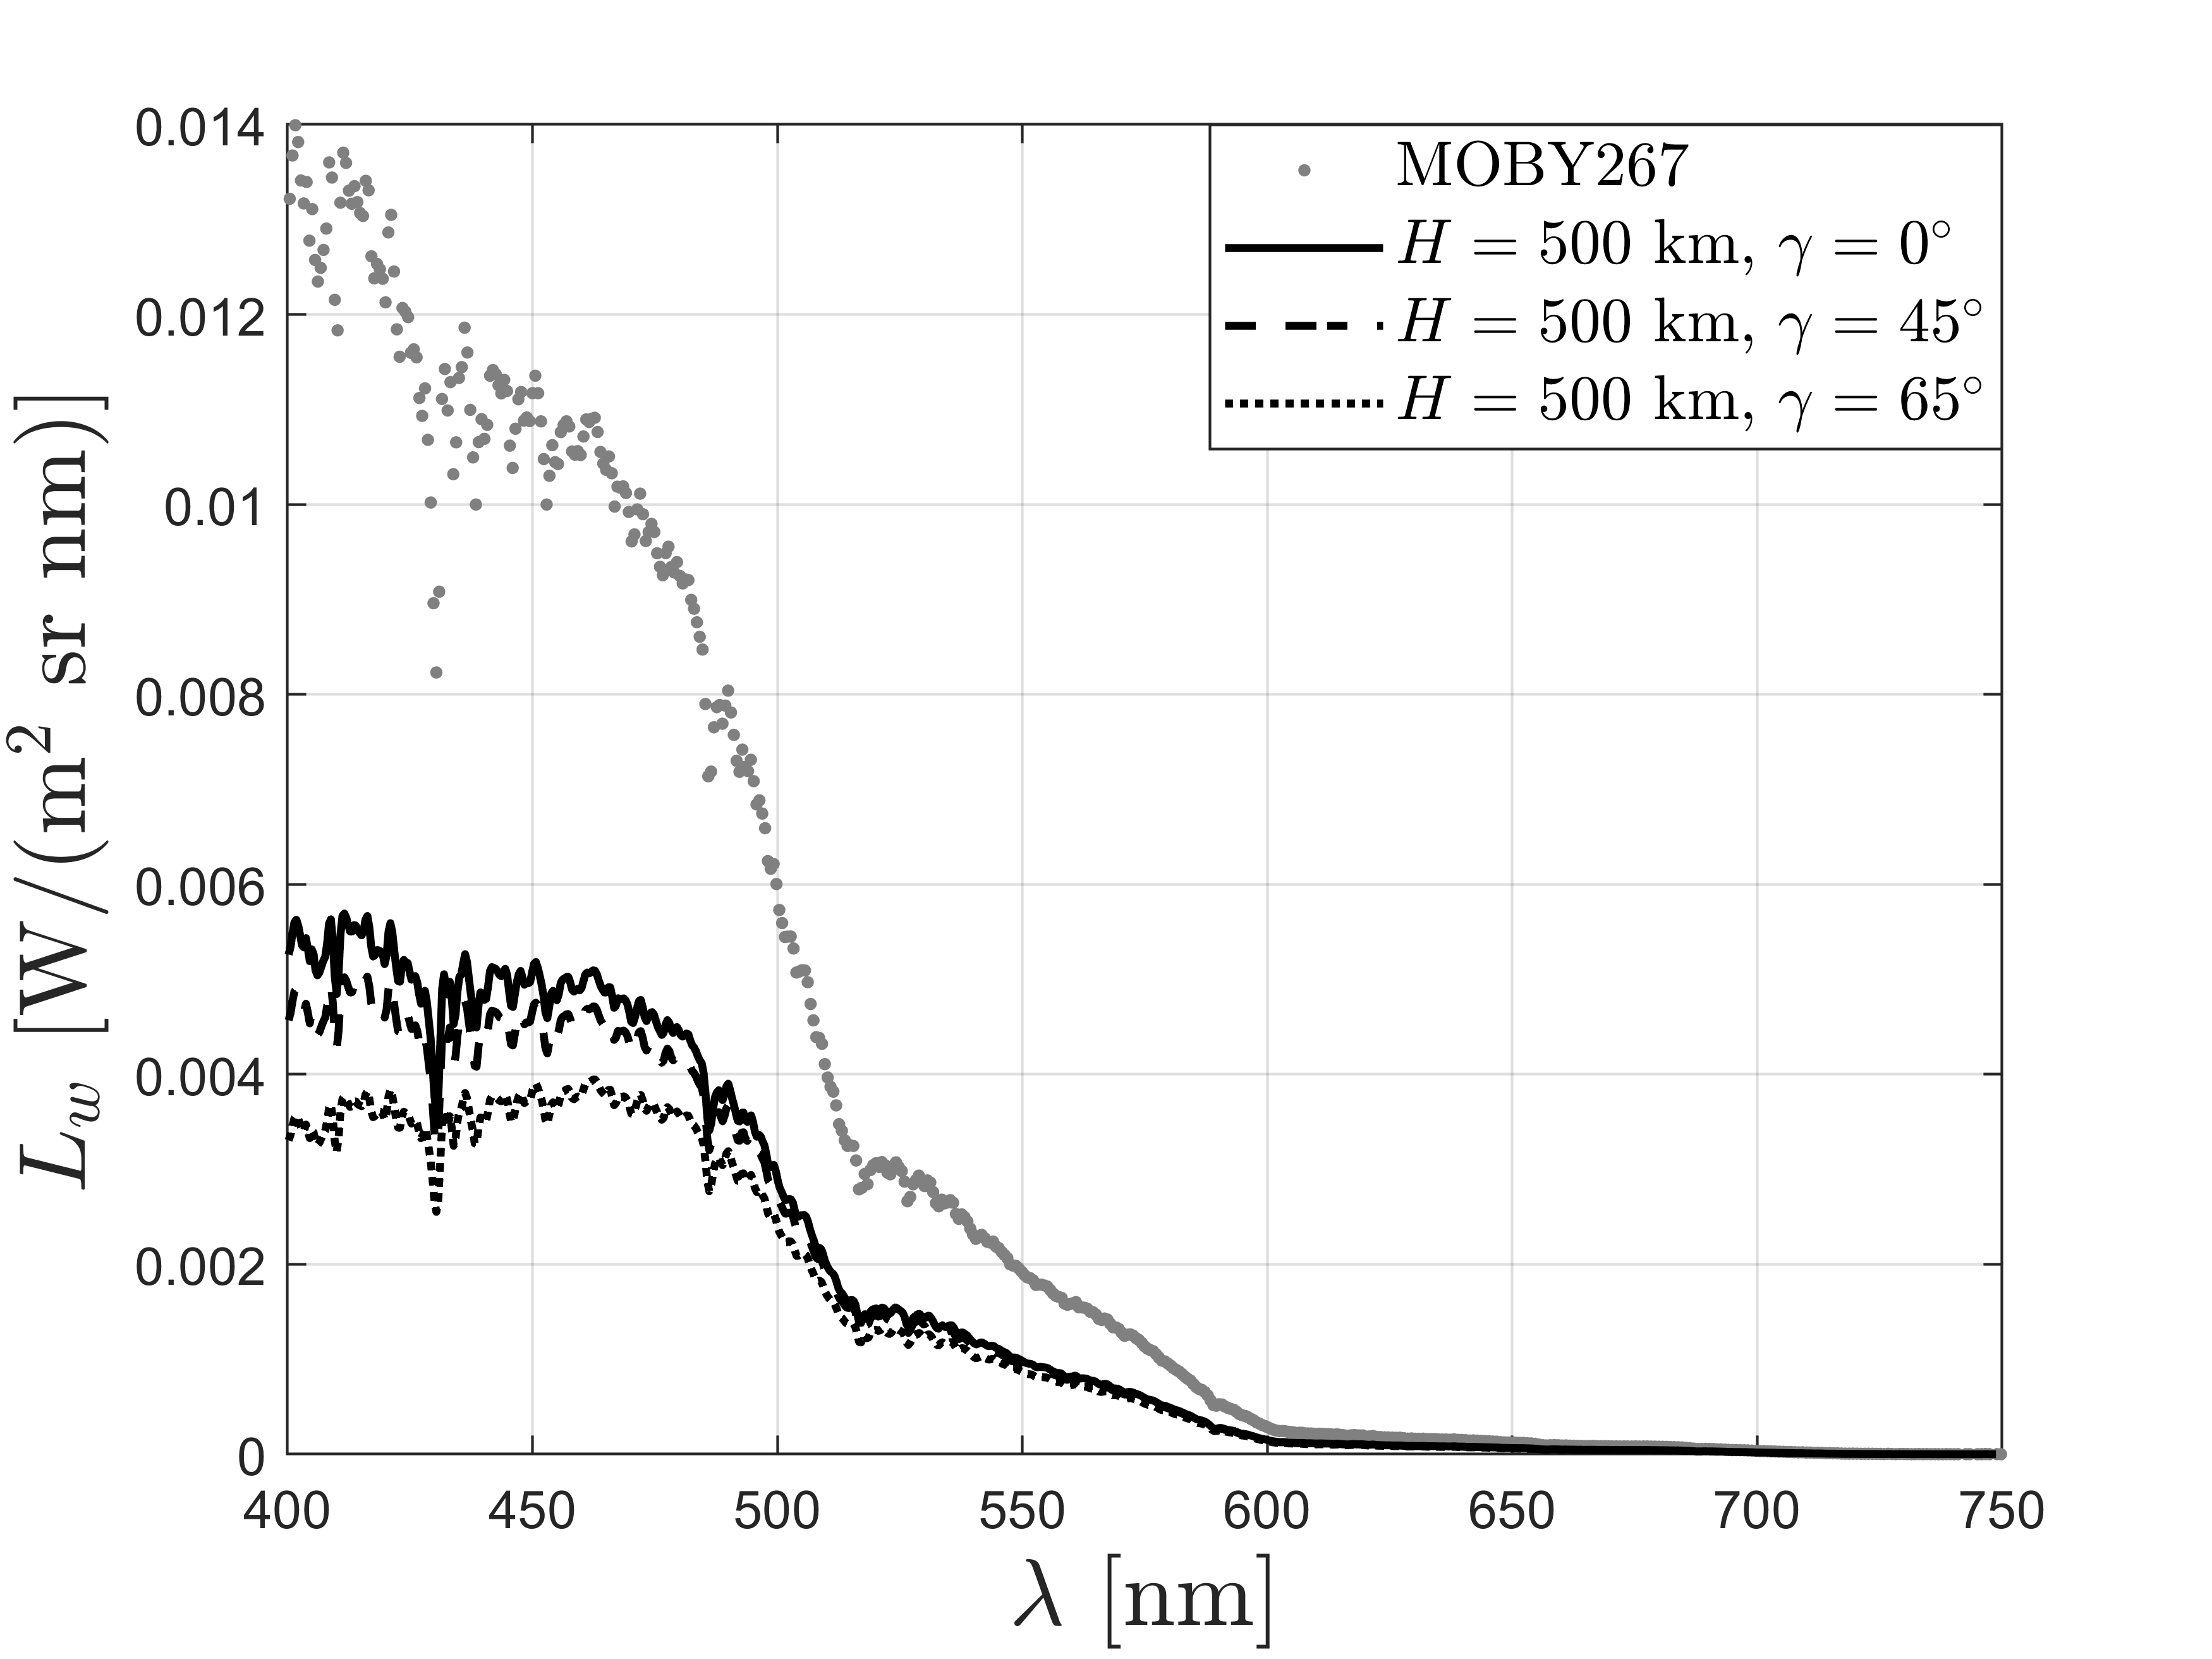
\includegraphics[width=0.45\textwidth]{figs/radiance.png}
  \caption{Water-leaving radiance $L_w$ measured by MOBY267 and estimated at ToA for different viewing angles $\gamma$.}
	\label{fig:signal}
\end{figure}
To simulate typical water conditions to be observed by HYPSO-1's hyperspectral imager and its corresponding estimate of SNR, we have used water-leaving radiance measurements from the Marine Optical BuoY (MOBY) with deployment number $267$ off the coast of Hawaii. The data sets are publicly available, mainly used for vicarious calibration of EO remote sensing data \cite{Clark2002}. The chosen measurements are time-stamped at 21:11:38 GMT on 3 July 2019 and a spline curve is fitted to the calibrated data in the wavelength range of $348.8391-749.7629 \hspace{3pt} \rm{nm}$ to match the resolution of the hyperspectral imager. Figure \ref{fig:signal} shows the point measurements and simulated water-leaving radiance for viewing angles $\gamma$ as seen at Top-of-Atmosphere (ToA), assuming that the water-leaving radiance diminishes due to the water refraction index and the atmospheric transmittance consisting of only the Rayleigh optical thickness \cite{Bucholtz1995}. 
% It is also assumed that photon flux is constant during the short exposure time $\tau$. 
% 12 binning, 160 binned pixels, 1936/12 = 160 pixels, 500/160=3.1 nm per binned pixel.
% \begin{figure}[htbp]
%   \centering
%       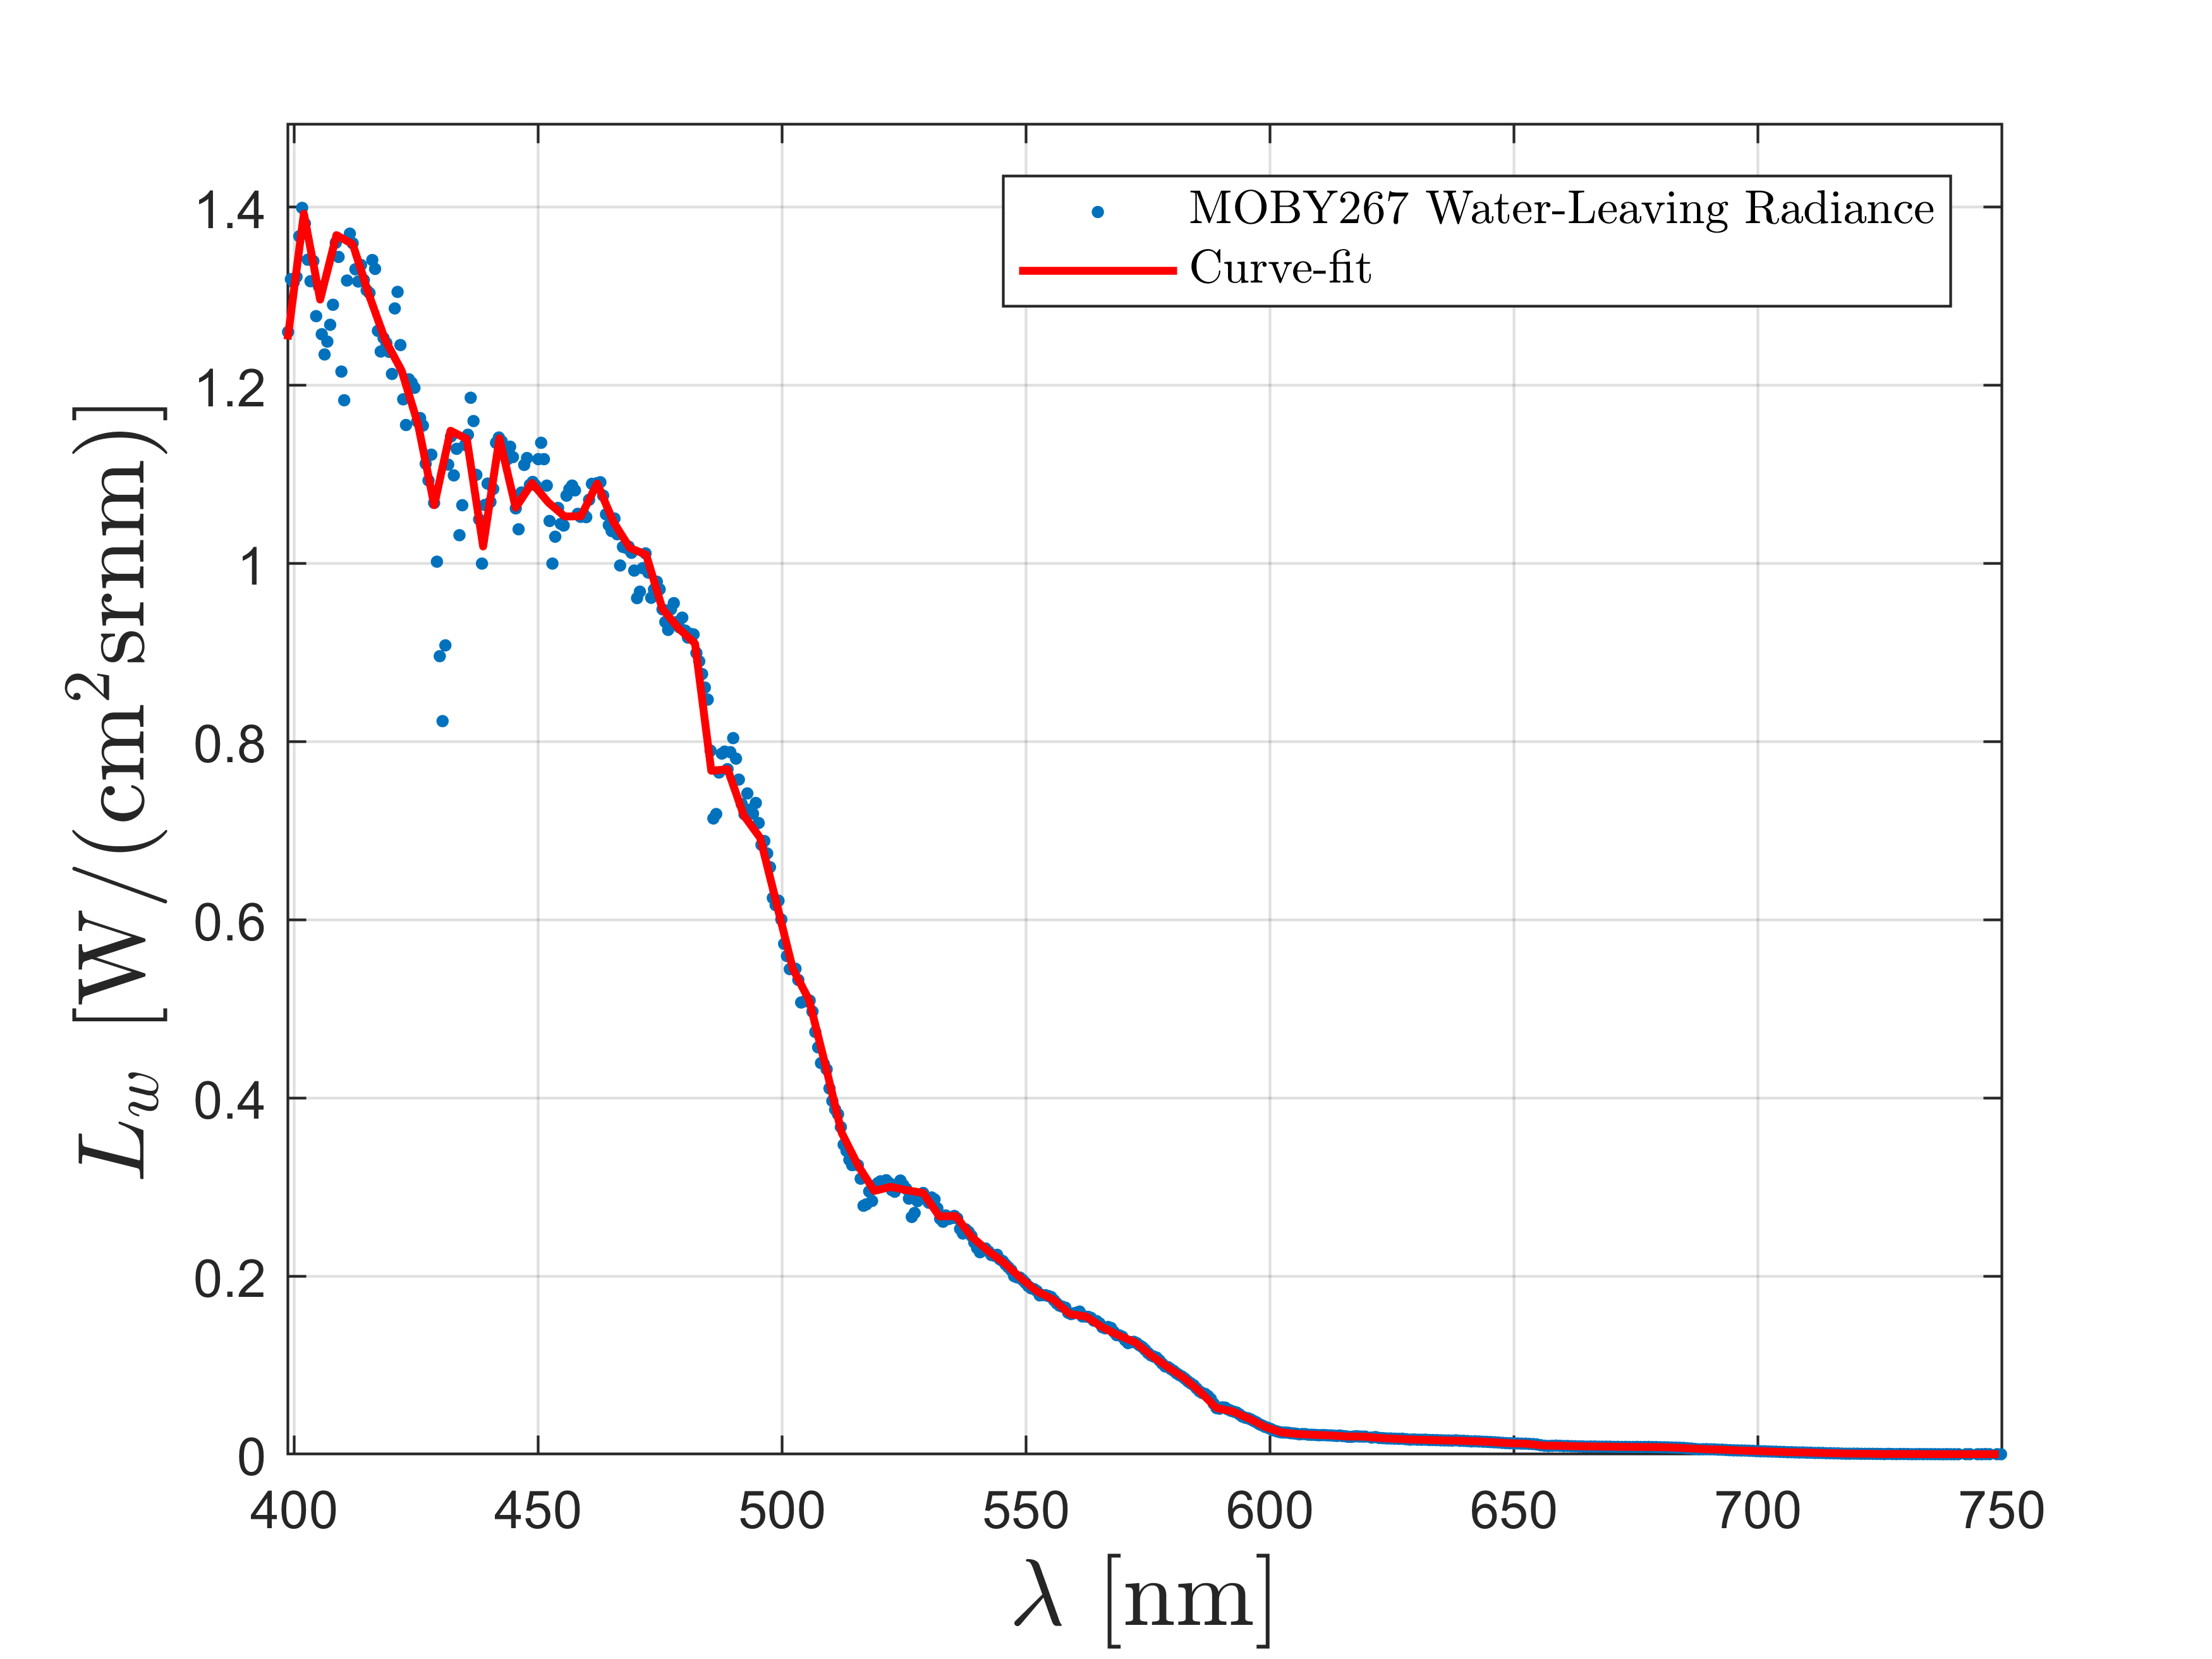
\includegraphics[width=0.45\textwidth]{figs/MOBY.png}
%   \caption{Water-leaving radiance data collected by MOBY. Red line shows a curve fit to the data at spectral resolution .}
% 	\label{fig:moby}
% \end{figure}
\begin{figure}[htbp]
  \centering
      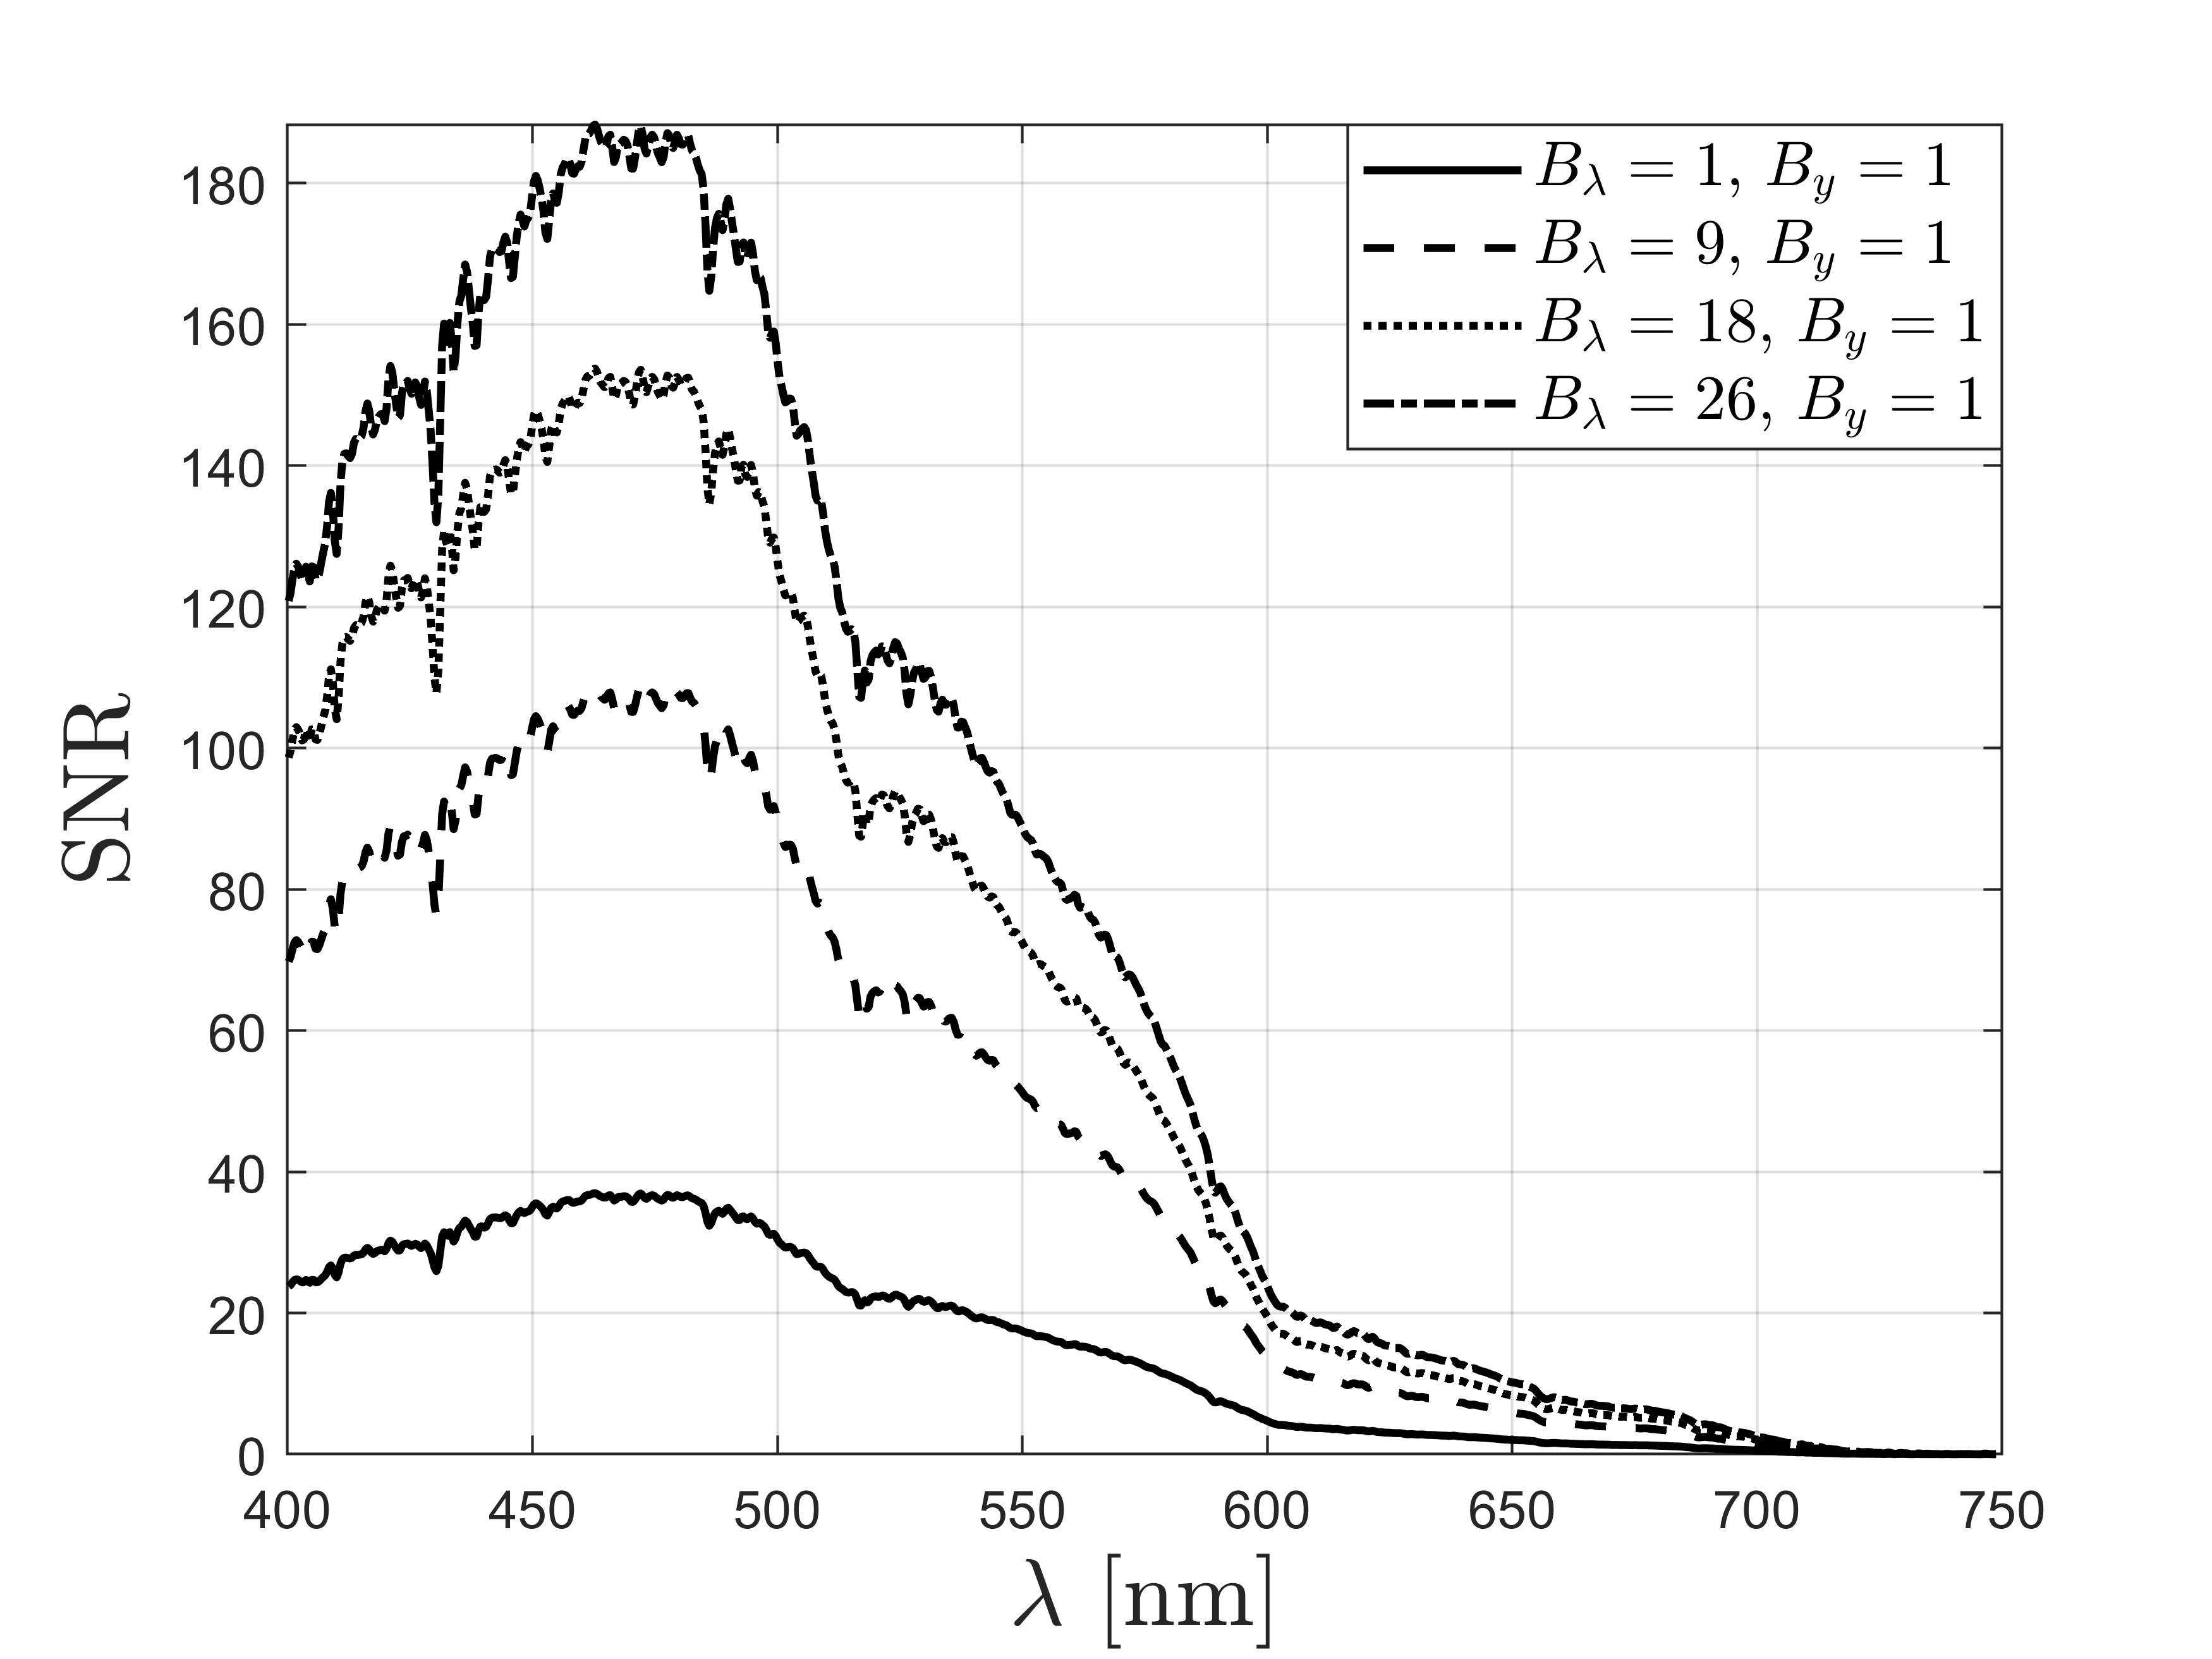
\includegraphics[width=0.45\textwidth]{figs/snr.png}
  \caption{SNR of $L_w$ as seen at ToA with selected number of binning operations per pixel.}
	\label{fig:fred_snr2}
\end{figure}

Using Eqs. (\ref{eq:photons}), (\ref{eq:photons2}) and (\ref{eq:snr}), Figure \ref{fig:fred_snr2} shows the estimated SNR in the $400-750\hspace{3pt} \rm{nm}$ spectral range for the hyperspectral imager sensing the radiance $L=L_w$ at ToA with $\gamma=0^{\circ}$ and $\tau=41.4 \hspace{3pt} \rm{ms}$. It is shown how binning  pixels in the spectral direction increases the SNR. With no binning and at $B_\lambda=9$ we have $BP=3.33 \hspace{3pt} \rm{nm}$ while $B_\lambda=18$ and $B_\lambda=26$ result in $BP=6.67 \hspace{3pt} \rm{nm}$ and $BP=10 \hspace{3pt} \rm{nm}$, respectively. 
% Blue curve shows SNR per unbinned pixel. Red curve shows SNR for $B_\lambda=N_w$ binned pixels along the spectral direction. Green curve shows SNR for binned pixels with $B_\lambda=3 \times N_w$ along the spectral direction to achieve $BP=10 \hspace{3pt} \rm{nm}$. Without binning in cross-track spatial dimension $B_y$, the optical spatial resolution of a pixel for this case is $\delta x \times \delta y = 500 \hspace{3pt} \rm{m} \times 57.65 \hspace{3pt} \rm{m}$. Magenta curve shows a square window of pixels $9\times 9$ with bandpass of $BP=3.33 \hspace{3pt} \rm{nm}$, that means $B_y=9$ pixels are binned in the spatial direction. Optical spatial resolution for this cases is $\delta x \times B_y\delta y = 500 \hspace{3pt} \rm{m} \times 518.65 \hspace{3pt} \rm{m}$.
It is worth mentioning that the simulated SNR does not take into account the total radiance at ToA which includes light due to predominantly aerosol scattering and sun reflection \cite{Franz2007}. Atmospheric scattering of the solar radiation into the hyperspectral imager's path will typically be 10 to 20 times larger at $500 \hspace{3pt} \rm{km}$ altitude \cite{Corson2008, Gao2012}. With this assumption, $20\cdot L_w$ or $\sqrt{20}$ times the highest SNR of $36.97$ at $463 \hspace{3pt} \rm{nm}$ would be approximately $\sqrt{20}\cdot36.97=165.33$ which is still below the saturation at SNR of $181.6$ for an unbinned pixel. Further, the effective SNR is expected to increase due to more overlapping frames during a slew maneuver. For an ideal slew maneuver with $\omega_y=0.754^{\circ}\rm{/s}$, rendering $12$ overlapping frames, results in up to $\sqrt{12}$ times higher SNR for an image pixel containing the same scene.
% For instance, when observing the radiance $L_w$ presented in Figure \ref{fig:signal} which gives the photon flux of $20703 \hspace{3pt} \rm{e^{-}/s}$ into each pixel assuming ToA radiance is 10 times larger, then the exposure time setting may be constrained to be $\tau<1.59 \hspace{3pt} \rm{s}$.

% For example, by binning $B_\lambda=3 N_\lambda = 26$ and keeping $B_y=1$ then the bandpass becomes $BP=10 \hspace{3pt} \rm{nm}$ and SNR at $495.5 \hspace{3pt} \rm{nm}$ increases with $73 \%$ compared to the case with $B_\lambda=N_\lambda=8.67$ and $BP=3.34 \hspace{3pt} \rm{nm}$. 
% Figure \ref{fig:fred_snr3} shows the calculated SNR of water-leaving target radiance for a square window of pixels $N_\lambda \times N_y = 26 \times 26$ and $BP=10 \hspace{3pt} \rm{nm}$. Optical spatial resolution for this case is $\delta x \times B_y \delta y = 500 \hspace{3pt} \rm{m} \times 1498.1 \hspace{3pt} \rm{m}$.
% \begin{figure}[htbp]
%   \centering
%       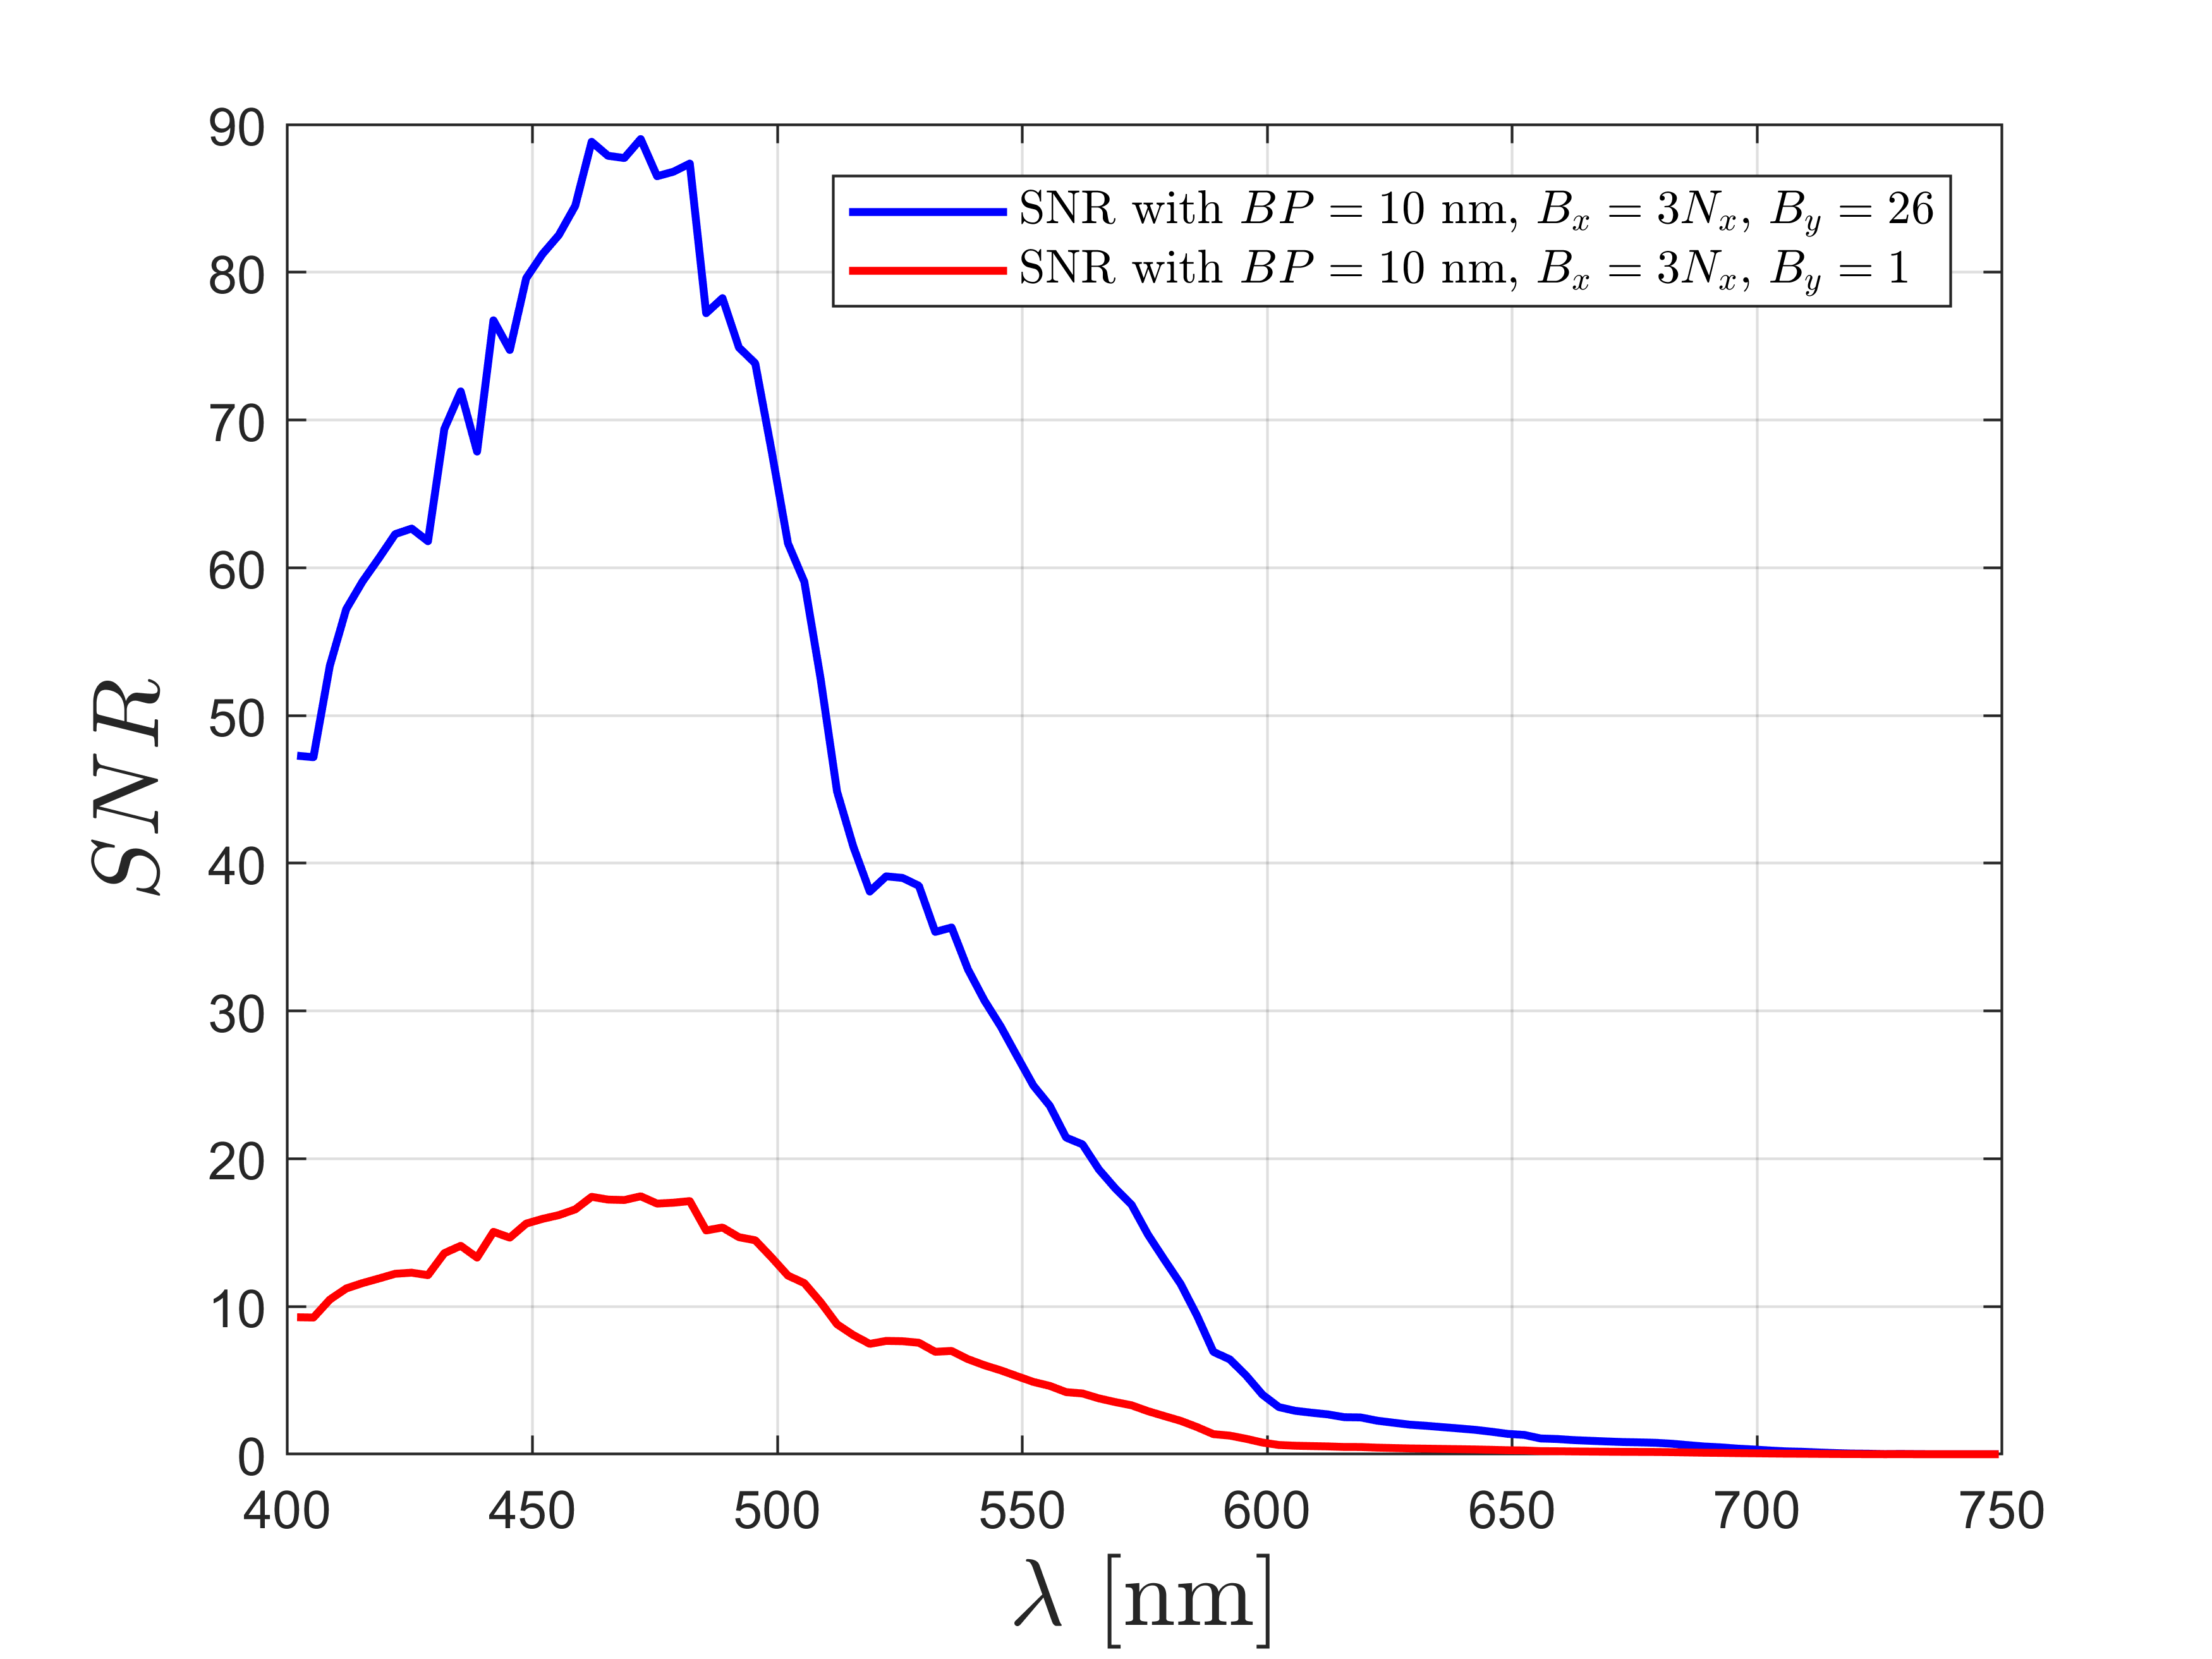
\includegraphics[width=0.45\textwidth]{figs/SNR_Fred2.png}
%   \caption{SNR for binned square window of pixels is shown in blue where $N_\lambda \times N_y = 26 \times 26$ and $BP=10 \hspace{3pt} \rm{nm}$. Red curve shows SNR for a window of pixels with $N_\lambda \times N_y = 26 \times 1$ and $BP=10 \hspace{3pt} \rm{nm}$.}
% 	\label{fig:fred_snr3}
% \end{figure}


% As shown in Fig. \ref{fig:snr_lambda}, if there are $13$ overlapping pixels, then SNR at $495.5 \hspace{3pt} \rm{nm}$ is 30.16 and increases with $261 \%$ compared to the case with unbinned pixels. Furthermore if there are four satellites with $13$ overlapping pixels at same altitude $500\hspace{3pt} \rm{km}$ then the SNR is 176.77 which is an increase of $621 \%$ compared to the case with non-overlapped pixels. SNR is then 1.017 at $619 \hspace{3pt} \rm{nm}$ while for non-overlapped case with unbinned pixels the SNR is only $0.2822$ at the same wavelength. If there are additional four pixels that overlap from four other satellites with same viewing angles, then SNR is $>1$ at $652.4 \hspace{3pt} \rm{nm}$.
% \begin{figure}[htbp]
%   \centering
%       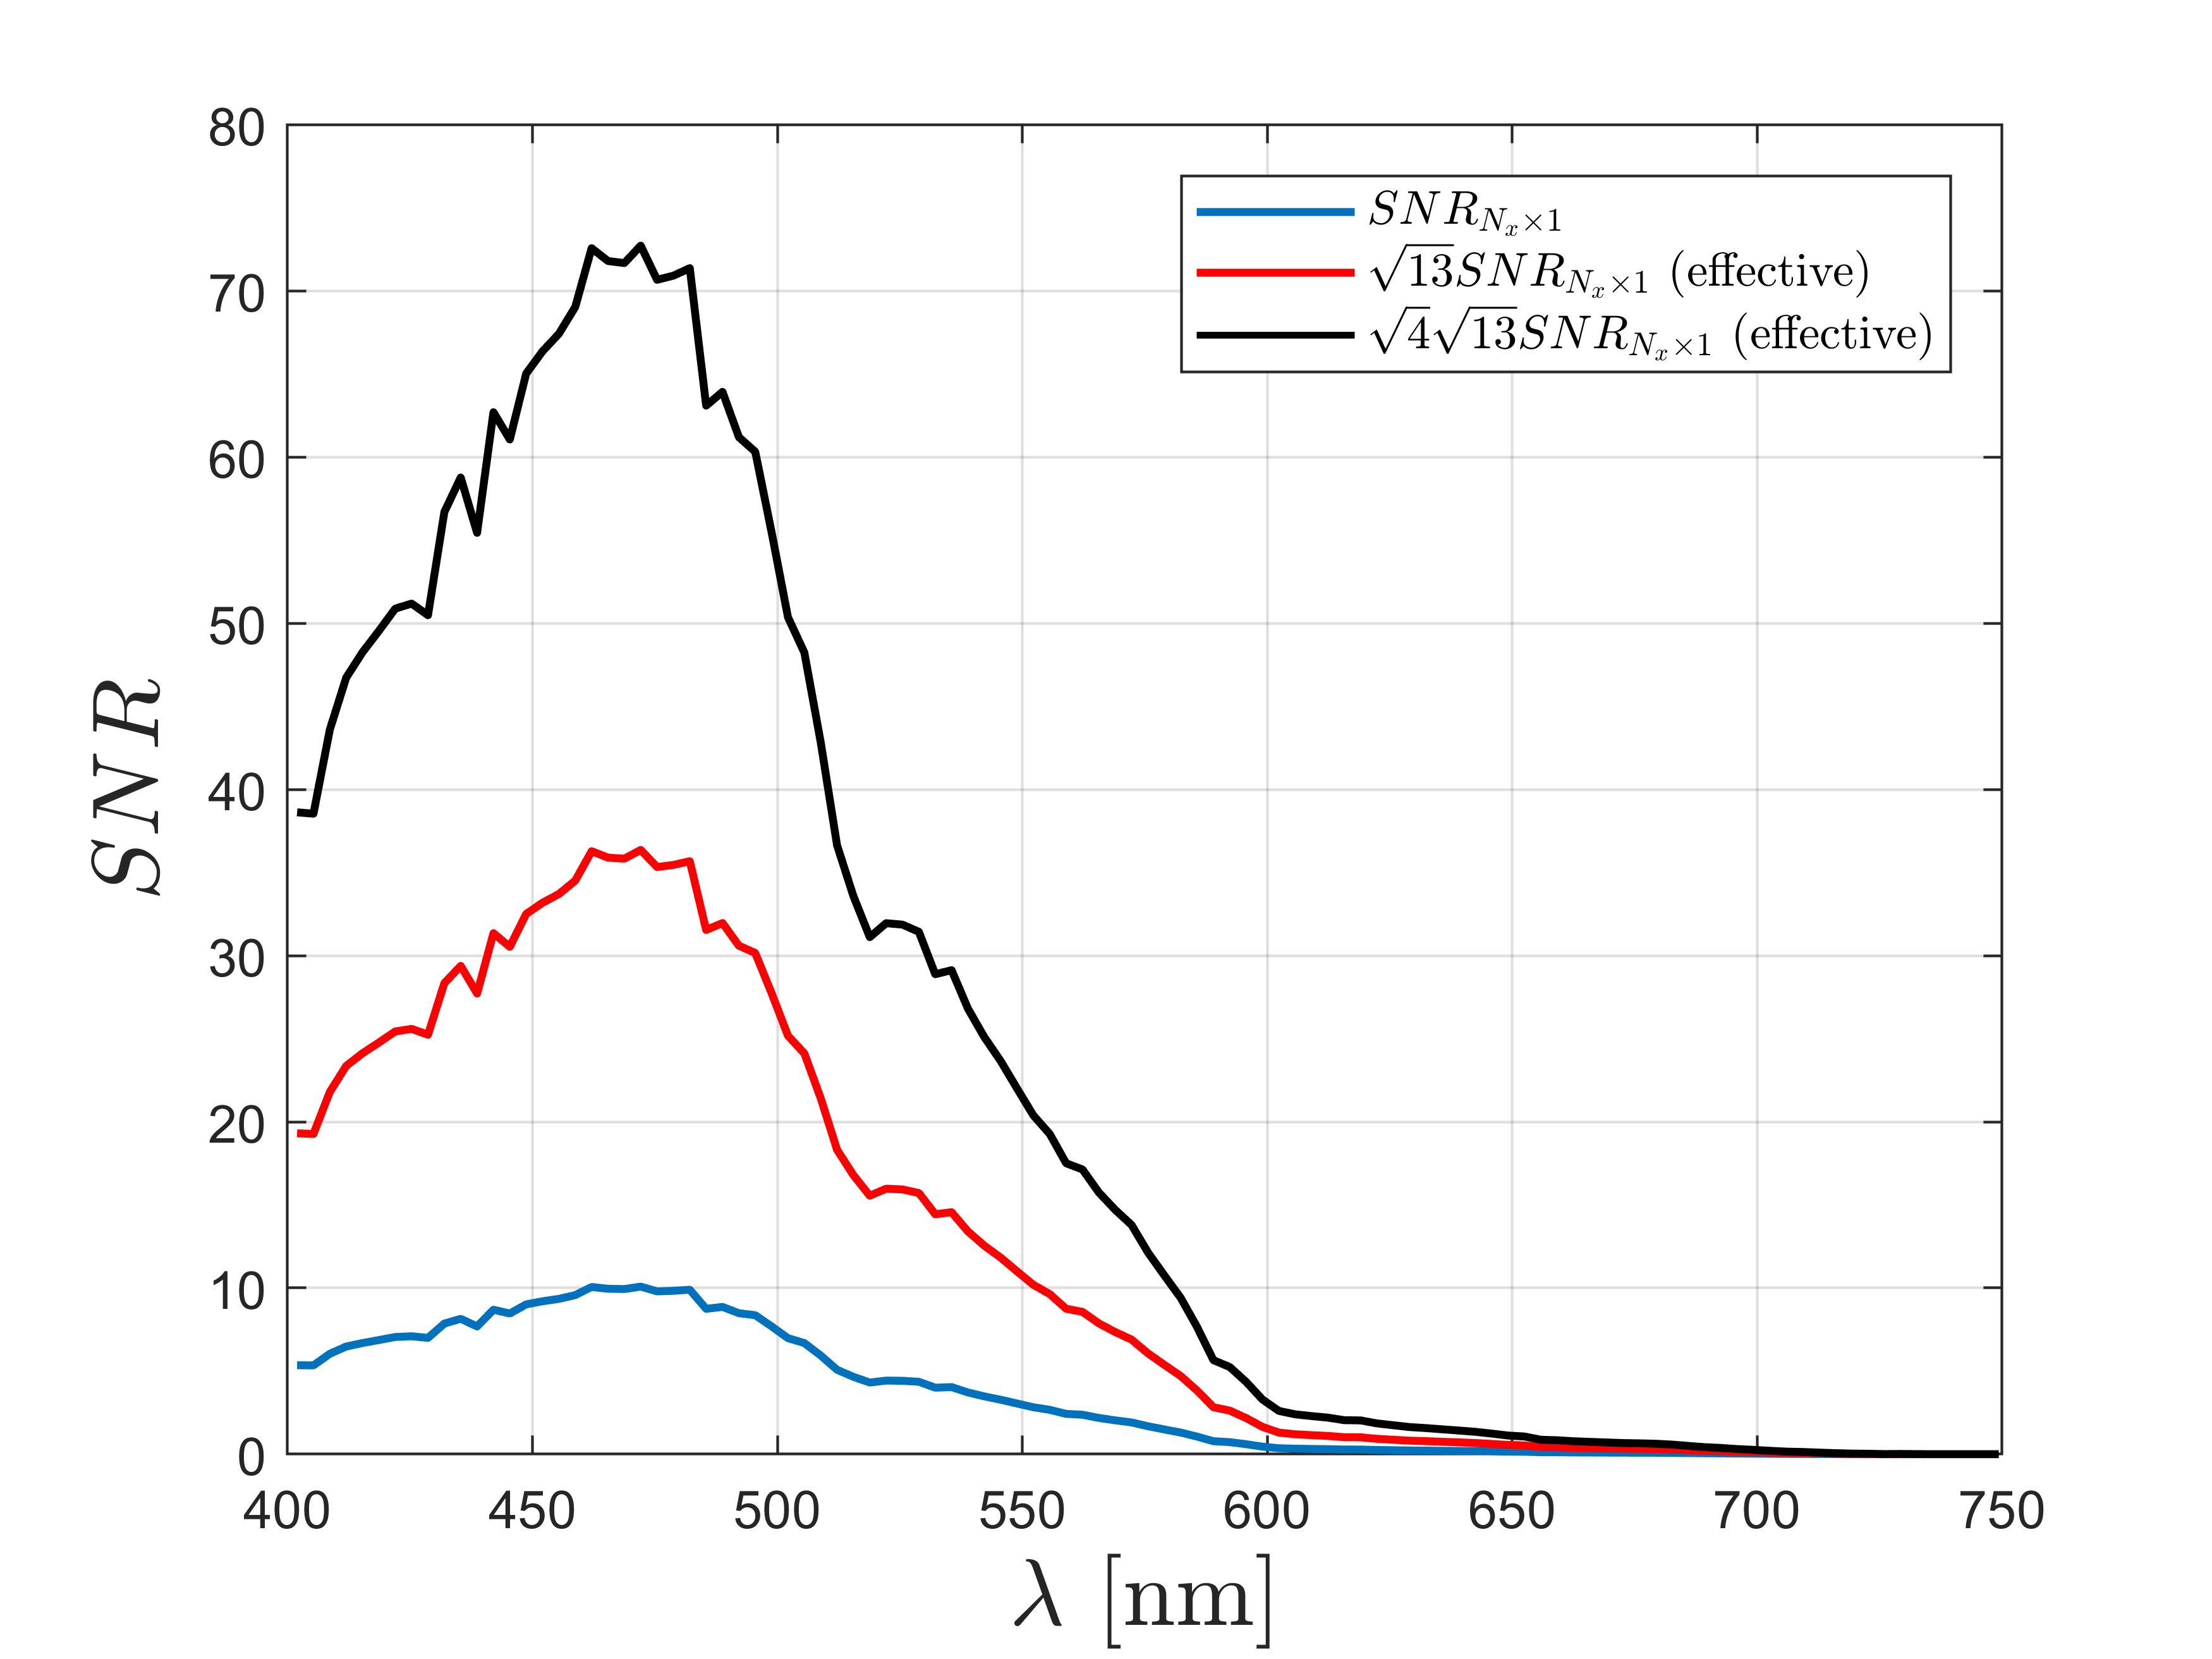
\includegraphics[width=0.45\textwidth]{figs/snr_lambda.png}
%   \caption{SNR in a pixel for a spacecraft HSI sensing the Earth water-leaving radiance $L_w$ at $\gamma=0^{\circ}$. The dashed red curve shows the effective SNR in the case of $13$ overlapping pixels. The dashed black curve shows effective SNR when 4 spacecraft are mapping the same target area with 13 overlapping pixels. Exposure time for all spacecraft are $\tau=25 \hspace{3pt} \rm{ms}$.}
% 	\label{fig:snr_lambda}
% \end{figure}